\documentclass[nojss]{jss}

% \VignetteIndexEntry{maxlogL: Maximum Likelihood estimation in R}
% \VignetteKeyword{Maximum likelihood estimation}
% \VignetteKeyword{Parameter estimation}

%% -- LaTeX packages and custom commands ---------------------------------------

%% recommended packages
\usepackage{thumbpdf,lmodern}
\usepackage{amsmath, bm}
\usepackage{amssymb}
\usepackage{subcaption}
\usepackage{float}
\usepackage{xcolor}

%% another package (only for this demo article)
\usepackage{framed}

%% new custom commands
\newcommand{\class}[1]{`\code{#1}'}
\newcommand{\fct}[1]{\code{#1()}}

%% For Sweave-based articles about R packages:
%% need no \usepackage{Sweave}



%% -- Article metainformation (author, title, ...) -----------------------------

%% - \author{} with primary affiliation
%% - \Plainauthor{} without affiliations
%% - Separate authors by \And or \AND (in \author) or by comma (in \Plainauthor).
%% - \AND starts a new line, \And does not.
\author{Jaime Mosquera Guti\'errez\\Universidad Nacional de Colombia
   \And Freddy Hern\'andez\\Universidad Nacional de Colombia}
\Plainauthor{Jaime Mosquera Guti\'errez, Second Author}

%% - \title{} in title case
%% - \Plaintitle{} without LaTeX markup (if any)
%% - \Shorttitle{} with LaTeX markup (if any), used as running title
\title{\pkg{maxlogL}: A general computational procedure for Maximum Likelihood estimation in \proglang{R}}
\Plaintitle{maxlogL: A general computational procedure for Maximum Likelihood estimation in R}
\Shorttitle{\pkg{maxlogL}: Maximum Likelihood estimation in \proglang{R}}

%% - \Abstract{} almost as usual
\Abstract{
  Maximum likelihood (ML) method is preferred among others because it
  produces consistent and efficient estimators. However, likelihood
  optimization processes frequently involve unwieldy mathematical
  expressions and it is necessary in some cases to implement distributions
  and constantly build (log-)likelihood functions in computing languages
  in order to get numerical solutions. We present \code{maxlogL}, a function
  contained in the \pkg{EstimationTools} package for ML parameter estimation
  of any probability function loaded in \proglang{R} with no need of special
  structures, given a data set. We show via simulation that the routine
  has good performance in estimating the parameters of three distributions
  (normal, ZIP and user-defined). Finally, we present two application
  examples with real data.
}

%% - \Keywords{} with LaTeX markup, at least one required
%% - \Plainkeywords{} without LaTeX markup (if necessary)
%% - Should be comma-separated and in sentence case.
\Keywords{Maximum likelihood estimation, parameter estimation, \proglang{R}, \pkg{EstimationTools}}
\Plainkeywords{Maximum likelihood estimation, parameter estimation, R, EstimationTools}

%% - \Address{} of at least one author
%% - May contain multiple affiliations for each author
%%   (in extra lines, separated by \emph{and}\\).
%% - May contain multiple authors for the same affiliation
%%   (in the same first line, separated by comma).
\Address{
  Jaime Mosquera Guti\'errez\\
  Universidad Nacional de Colombia\\
  School of Statistics\\
  Faculty of Sciences\\
  Universidad Nacional de Colombia\\
  Cra. 65 \#59a-110\\
  Medell\'in, Colombia\\
  E-mail: \email{jmosquerag@unal.edu.co}\\
  % URL: \url{https://eeecon.uibk.ac.at/~zeileis/}
}

\begin{document}

%% -- Introduction -------------------------------------------------------------

%% - In principle "as usual".
%% - But should typically have some discussion of both _software_ and _methods_.
%% - Use \proglang{}, \pkg{}, and \code{} markup throughout the manuscript.
%% - If such markup is in (sub)section titles, a plain text version has to be
%%   added as well.
%% - All software mentioned should be properly \cite-d.
%% - All abbreviations should be introduced.
%% - Unless the expansions of abbreviations are proper names (like "Journal
%%   of Statistical Software" above) they should be in sentence case (like
%%   "generalized linear models" below).

\section{Introduction} \label{sec:intro}

Parameter estimation for probability density functions or probability mass functions is a central problem in statistical analysis and applied sciences because it allows to build predictive models and make inferences. Traditionally
this problem has been tackled by means of likelihood maximization, as it was introduced by \cite{Fisher1912}. The method consists on performing an optimization through first derivative of the log-likelihood function and solve the outcoming system of equations. Despite its validity for any probability distribution, there exist a vast variety of them with cumbersome derivatives which produce non-linear systems of equations, therefore it is necessary to implement numerical methods and develop computational algorithms to find a solution.

\proglang{R} \citep{R2019} is a free language developed for statistical computing and equipped with unconstrained and box-constrained general-purpose optimization tools in \pkg{base} package: \cite{Fox1978} developed the function \code{nlminb} for optimization using PORT (portable \proglang{Fortran} programs for numerical computation) routines; \cite{Nash1979} implemented \code{optim}, a function that performs optimization based on three algorithms: (1) \cite{Nelder1965}, (2) quasi-Newton (\code{BFGS}) and (3) conjugate-gradient (\code{CG}). Either the former or the latter is implemented, users must take a distribution included in any package or create their own function otherwise and then write the likelihood.

On the other hand, \proglang{R} posses an extensive number of libraries (add-ons) in order to enhance its capabilities, e.g \pkg{gamlss}  package \citep{Stasinopoulos+Rigby:2007} for fitting generalized additive models for location, scale and shape. It is possible to carry out parameter estimation with an empty regression model of any distribution implemented as a \code{gamlss.family} structure. Visit \cite{Stasinopoulos2017} for more details.

In this paper, we introduce the function \code{maxlogL}, which is capable of applying maximum likelihood estimation based on optimization through \code{optim} or \code{nlminb} only with the density/mass function defined as usual in \proglang{R}. The user could define its own distribution or use whichever existing in any package. The remainder of the article defines the maximization problem mathematically and computationally. Then, we present a simulation study to evaluate the performance of \code{maxlogL} with data generated from normal, ZIP and user-defined distributions. Finally, we give an application with a real data set and present some conclusions.

%% -- Manuscript ---------------------------------------------------------------

%% - In principle "as usual" again.
%% - When using equations (e.g., {equation}, {eqnarray}, {align}, etc.
%%   avoid empty lines before and after the equation (which would signal a new
%%   paragraph.
%% - When describing longer chunks of code that are _not_ meant for execution
%%   (e.g., a function synopsis or list of arguments), the environment {Code}
%%   is recommended. Alternatively, a plain {verbatim} can also be used.
%%   (For executed code see the next section.)

\section{Maximum Likelihood estimation} \label{sec:MLE}

Let be $\boldsymbol{y}^\top=(y_1,y_2,...,y_n)$ a random sample with $n$ observations drawn from a population with distribution $f(\cdot|\boldsymbol{\theta})$, with $\boldsymbol{\theta}$ a vector of parameters. The likelihood function of $\boldsymbol{\theta}$ is

\begin{equation}
L(\boldsymbol{\theta}|\bm{y}) = \prod_{i=1}^{n}
f(y_i|\boldsymbol{\theta}).
\end{equation}

The method of ML finds the parameter values that makes data more probable. It is achieved by computing a vector $\boldsymbol{\hat{\theta}}$ such that

\begin{equation} \label{maxim}
\hat{\boldsymbol{\theta}} = \underset{\bm{\theta} \in \Theta}{\arg\max} \text{ } L(\boldsymbol{\theta}|\bm{y}).
\end{equation}

It is usual to perform maximization of log-likelihood function, i.e. $l(\boldsymbol{\theta}|\bm{y})=\log L(\boldsymbol{\theta}|\bm{y})$. The variance-covariance matrix of ML estimators is given by

\begin{equation}
Var(\hat{\boldsymbol{\theta}}) = I^{-1}(\hat{\boldsymbol{\theta}}) = C(\hat{\boldsymbol{\theta}}),
\end{equation}

where $I(\hat{\boldsymbol{\theta}})$ is the Fisher Information Matrix. The standard errors can be calculated as the square root of the diagonal elements of matrix $C$ \citep{Pawitan2013}%. Hence, the standard error of estimates is computed with the following expression

\begin{equation}
S.E(\hat{\boldsymbol{\theta}}) = \sqrt{C_{jj}(\hat{\boldsymbol{\theta}})}.
\end{equation}

The \proglang{R} function presented here calculates $l(\boldsymbol{\theta}|\bm{y})$ computationally, and computes standard errors from Hessian matrix.

\section{Basic usage and features}

Our \code{maxlogL} function is a S3 object of class \code{maxlogL}. It is included in \pkg{EstimationTools}, a package available from the Comprehensive R Archive Netwrok (CRAN) \url{https://cran.r-project.org/package=EstimationTools}. It can be downloaded and loaded in global environment typing the following instructions in the console:

\begin{Schunk}
\begin{Sinput}
R> install.packages("EstimationTools")
R> library(EstimationTools)
\end{Sinput}
\end{Schunk}

With \code{maxlogL} we provide a flexible implementation of ML estimation. It cab be executed stating its most important arguments

\begin{Schunk}
\begin{Sinput}
R> maxlogL(x, dist, optimizer, lower = NULL, upper = NULL)
\end{Sinput}
\end{Schunk}

where the argument \code{x} is a vector with data to be fitted, \code{dist} corresponds to the probability density/mass function of the working distribution, whereas \code{upper} and \code{lower} are limits used when user selects box-constrained algorithms. \code{maxlogL} is a wrapper function specifically developed for ML estimation, which allows to implement any of \code{optim} algorithms for optimization or \code{nlminb} routine for unconstrained or box-constrined optimization through the argument \code{optimizer}.

\pkg{EstimationTools} package provides a \code{summary} method for class \code{maxlogL}, which displays AIC (Akaike Information Criterion), BIC (Bayesian Information Criterion), ML estimates and its standard error. The method also reports the optimization routine selected by the user and the method used for computation of standard error. There are three methods available: \code{hessian} function from \pkg{numDeriv} package, calculation with \code{optim} (setting the argument \code{hessian = TRUE} and bootstrap calculation, with \code{boot} function of \pkg{boot} package \citep{Davison1997, Canty2017}.

Hence, for non-censorship fitting the user must pass a vector with data and specify a probability distribution function available in \proglang{R}. For example, fitting a sample generated from a normal distribution, $Z \sim \text{NO}(\mu=10,\: \sigma^2=1)$, could be done with the next command lines:

\begin{Schunk}
\begin{Sinput}
R> set.seed(1000)
R> z <- rnorm(n = 1000, mean = 10, sd = 1)
R> fit1 <- maxlogL(x = z, dist = 'dnorm', start=c(2, 3),
+                  lower=c(-15, 0), upper=c(15, 10))
R> summary(fit1)
\end{Sinput}
\begin{Soutput}
---------------------------------------------------------------
Optimization routine: nlminb 
Standard Error calculation: Hessian from optim 
---------------------------------------------------------------
       AIC      BIC
  2804.033 2800.033
---------------------------------------------------------------
     Estimate  Std. Error
mean   9.98752     0.0310
sd     0.98126     0.0219
-----
\end{Soutput}
\end{Schunk}

The \code{link} argument is a list with entries \code{fun} and \code{over}, which specify the link functions applied and the name of linked parameters in probability function implemented in \proglang{R} respectively. The estimation performed above can be carried out applying logarithm link funcion to $\sigma$, avoiding problems of estimation in the boundary of parametric space. The usage is illustrated in the following code snippet:

\begin{Schunk}
\begin{Sinput}
R> fit2 <- maxlogL(x = z, dist = 'dnorm',
+                  link = list(over = "sd", fun = "log_link"))
R> summary(fit2)
\end{Sinput}
\begin{Soutput}
---------------------------------------------------------------
Optimization routine: nlminb 
Standard Error calculation: Hessian from optim 
---------------------------------------------------------------
       AIC      BIC
  2804.033 2800.033
---------------------------------------------------------------
     Estimate  Std. Error
mean   9.98752     0.0310
sd     0.98126     0.0219
-----
\end{Soutput}
\end{Schunk}

The user can apply link functions to more than one parameter of the distribution:

\begin{Schunk}
\begin{Sinput}
R> fit3 <- maxlogL(x = z, dist = 'dnorm',
+                  link = list(over = c("mean", "sd"),
+                              fun = c("log_link", "log_link")))
R> summary(fit3)
\end{Sinput}
\begin{Soutput}
---------------------------------------------------------------
Optimization routine: nlminb 
Standard Error calculation: Hessian from optim 
---------------------------------------------------------------
       AIC      BIC
  2804.033 2800.033
---------------------------------------------------------------
     Estimate  Std. Error
mean   9.98752     0.0310
sd     0.98126     0.0219
-----
\end{Soutput}
\end{Schunk}

Other link functions available are logit and negative inverse, which must be specified as \code{"logit_link"} and \code{"NegInv_link"}. On the other hand, \code{maxlogL} allows to define fixed known parameters, e.g., the sample size $n$ in estimation of success proportion in a binomial distribution $N \sim \text{BI}(p=0.3, \: n=10)$. This parameters can be specified with \code{fixed} argument, which is a list that stores the fixed parameters value specified by their names

\begin{Schunk}
\begin{Sinput}
R> set.seed(100)
R> N <- rbinom(n = 100, size = 10, prob = 0.3)
R> phat <- maxlogL(x = N, dist = 'dbinom', fixed = list(size = 10),
+                  link = list(over = "prob", fun = "logit_link"))
R> summary(phat)
\end{Sinput}
\begin{Soutput}
---------------------------------------------------------------
Optimization routine: nlminb 
Standard Error calculation: Hessian from optim 
---------------------------------------------------------------
       AIC      BIC
  334.9805 334.9805
---------------------------------------------------------------
     Estimate  Std. Error
prob     0.312     0.0147
-----
\end{Soutput}
\end{Schunk}

As can be seen, the procedure applies the inverse of the link function to return the parameter to the original scale.

\section{Simulation Study}

In this section we simulated ML estimation with some distributions with \code{maxlogL}.

\subsection{Existing distributions}
We simulated the following two types of random variables: $X \sim \text{NO}(\mu=5,\: \sigma^2=4)$ with sample sizes $n \in \lbrace 3,...,400 \rbrace$ and $Y \sim \text{ZIP}(\lambda=6,\: \pi=0.08)$ with $n \in \lbrace 3,...,500 \rbrace$. We performed 1000 replications of each sample size.

\subsection{User-defined distribution}
Additionally, we simulated $W \sim \text{EEB}(\mu=0.5,\: \sigma=1, \nu=1.5, m=10)$ with $n \in \lbrace 3,...,1000 \rbrace$ (an exponentiated exponential binomial distribution, proposed by \cite{Bakouch2012}). As the previous case, we performed 1000 replications of each sample size. Probability density function of EEB distribution is given by the following expression:

\begin{equation} \label{EEBf}
  f(w|\mu, \sigma, \nu, m) = \frac{\sigma\nu\mu m}{1-(1-\mu)^m} \left(1 - e^{-\sigma w} \right)^{\nu-1} \left[ 1 - \mu\left(1 - e^{-\sigma w} \right)^\nu \right]^{m-1},
\end{equation}

with $w>0$, $\mu \in (0,1)$, $\sigma, \nu>0$ and $m$ an integer such that $m \geq 1$. We took this distribution as the user-defined by implementing it as an proglang{R} function, as is customary. Note that argument \code{size} corresponds to parameter $m$ in equation (\ref{EEBf}):

\begin{Schunk}
\begin{Sinput}
R> dEEB <- function(x, mu = 0.5, sigma = 1, nu = 1.5, size = 10,
+                   log = FALSE){
+    if (any(x<0))
+      stop(paste("x must greater than zero", "\n", ""))
+    if (any(mu < 0) | any(mu > 1))
+      stop(paste("mu must be between 0 and 1", "\n", ""))
+    if (any(sigma<=0 ))
+      stop(paste("sigma must be greater than zero", "\n", ""))
+    if (any(nu<=0 ))
+      stop(paste("nu must be greater than zero", "\n", ""))
+  
+    loglik <- log(sigma * nu * size *  mu) - sigma * x +
+              (nu - 1) * log(1 - exp(-sigma * x)) -
+              log(1 - (1 - mu)^size) +
+              (size - 1) * log(1 - mu * (1 - exp(-sigma * x))^nu)
+    if (log == FALSE)
+      density <- exp(loglik) else density <- loglik
+    return(density)
+  }
\end{Sinput}
\end{Schunk}



\begin{figure}[H]
    \begin{subfigure}[h]{0.49\textwidth}
        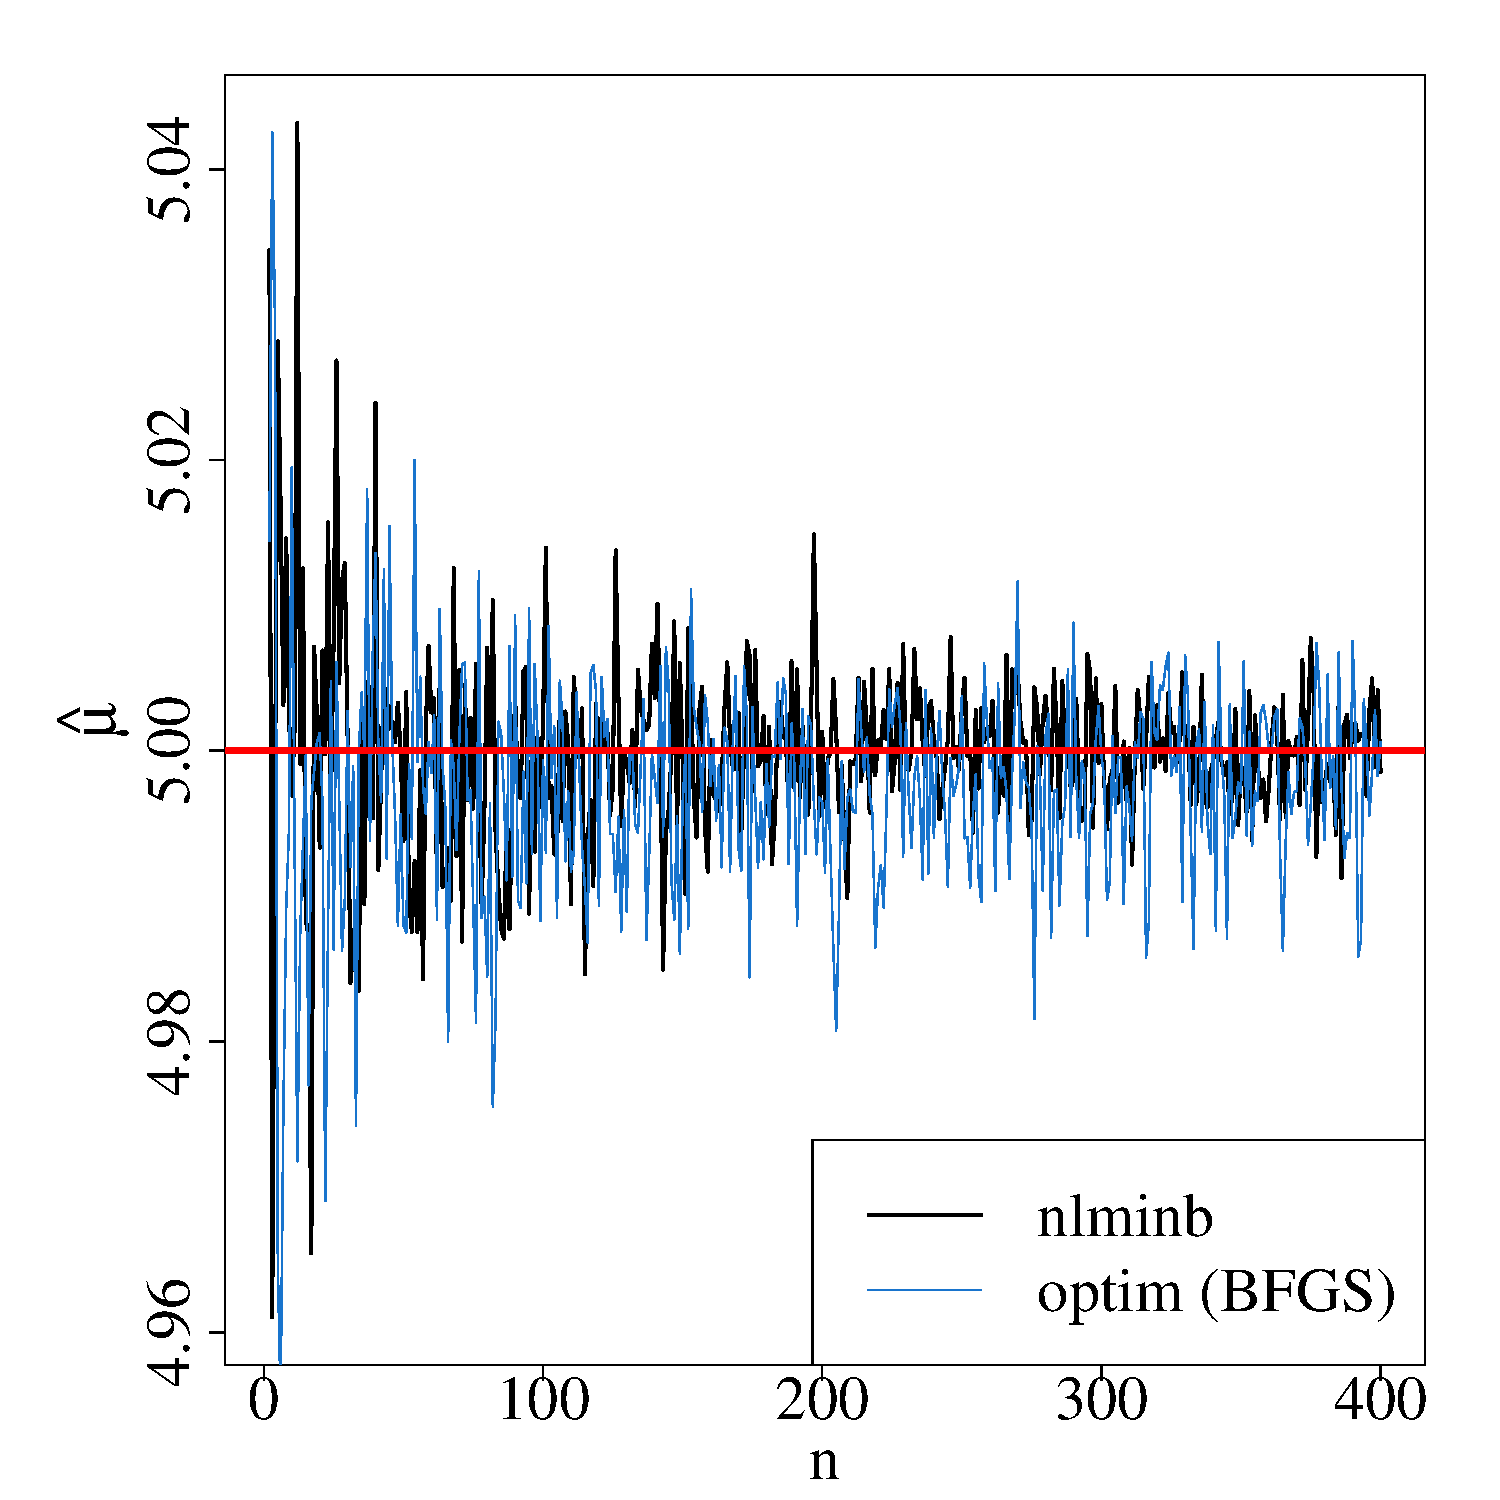
\includegraphics[width=\textwidth]{article-norm_a}
        \caption{\label{fig:norma}}
    \end{subfigure}
    \begin{subfigure}[h]{0.49\textwidth}
        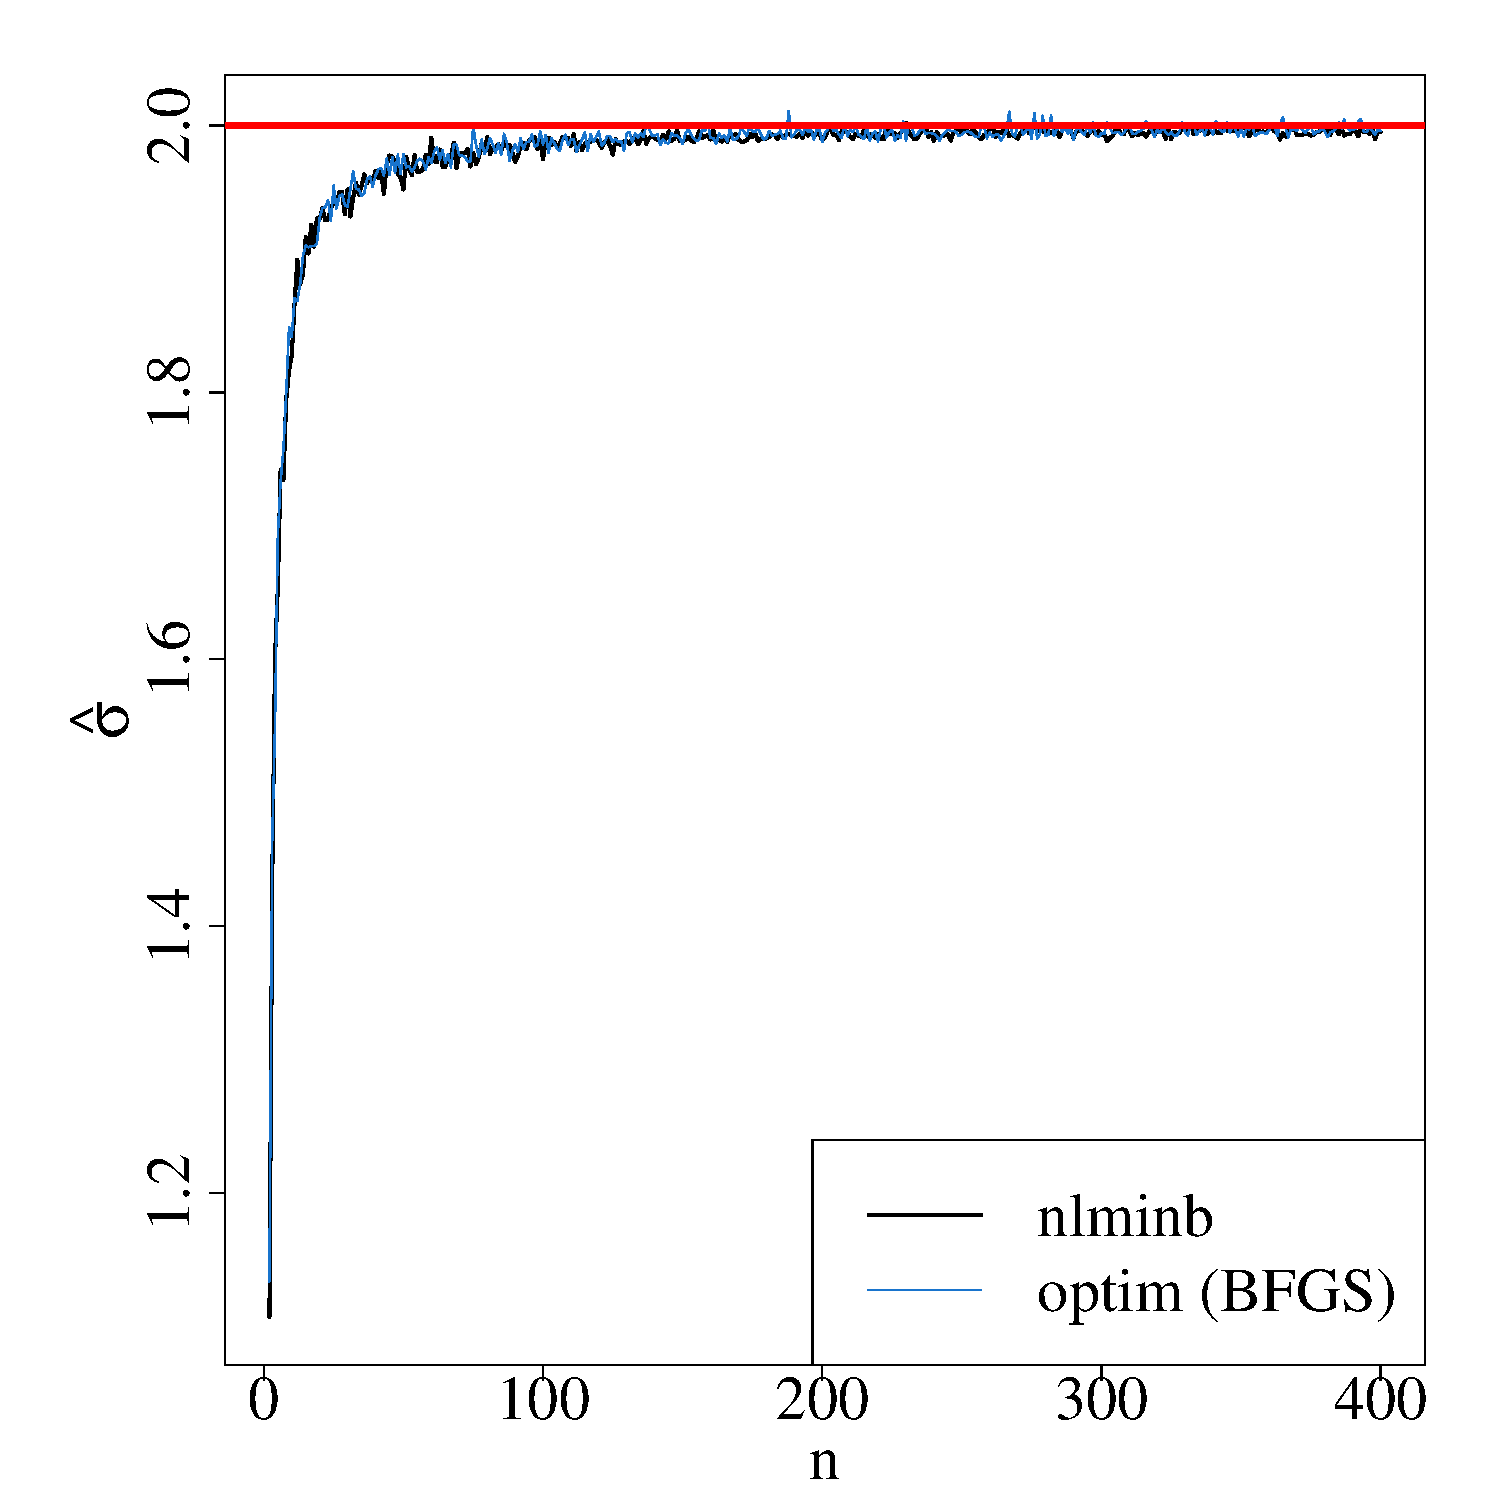
\includegraphics[width=\textwidth]{article-norm_b}
        \caption{\label{fig:normb}}
    \end{subfigure}
\caption{\label{fig:norm} Mean value for (a) location parameter $\hat{\mu}$ and (b) scale parameter $\hat{\sigma}$ versus sample size $n$ in normal distribution based on 1000 replications. Horizontal red lines are the true value of the parameters.}
\end{figure}
% {\color{white} Jaime} \nolinebreak[4]

\section{Results}\label{sec:results}

The results of Monte Carlo study for the three distributions mentioned are presented in Figure \ref{fig:norm} above, and Figures \ref{fig:EEB} and \ref{fig:ZIP} below. All the plots show that the mean estimates tend to the true value of the parameter as the sample size increases, as is expected under regularity conditions.




\begin{figure}[H]
  \centering
    \begin{subfigure}[h]{0.49\textwidth}
        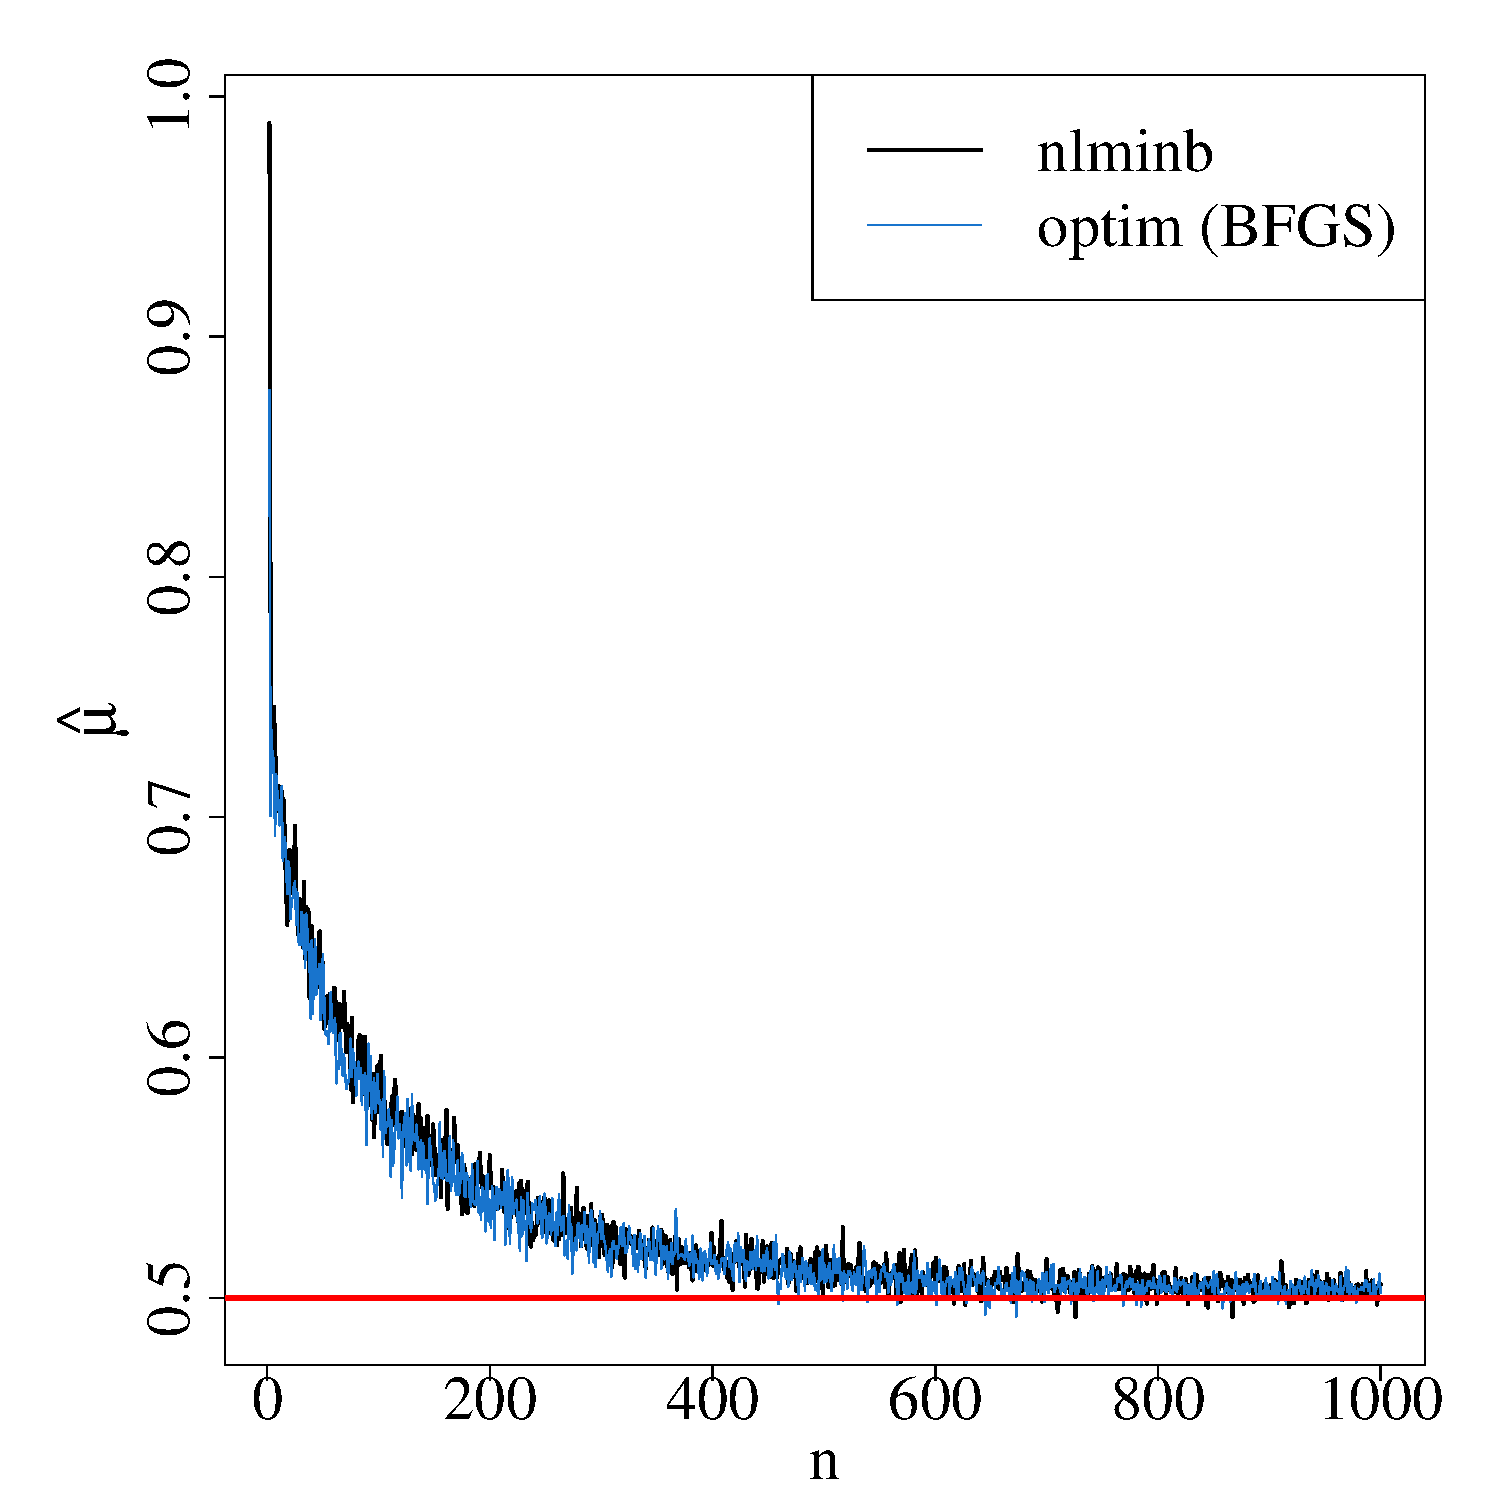
\includegraphics[width=\textwidth]{article-EEBa}
        \caption{\label{fig:EEBa}}
    \end{subfigure}
    \begin{subfigure}[h]{0.49\textwidth}
        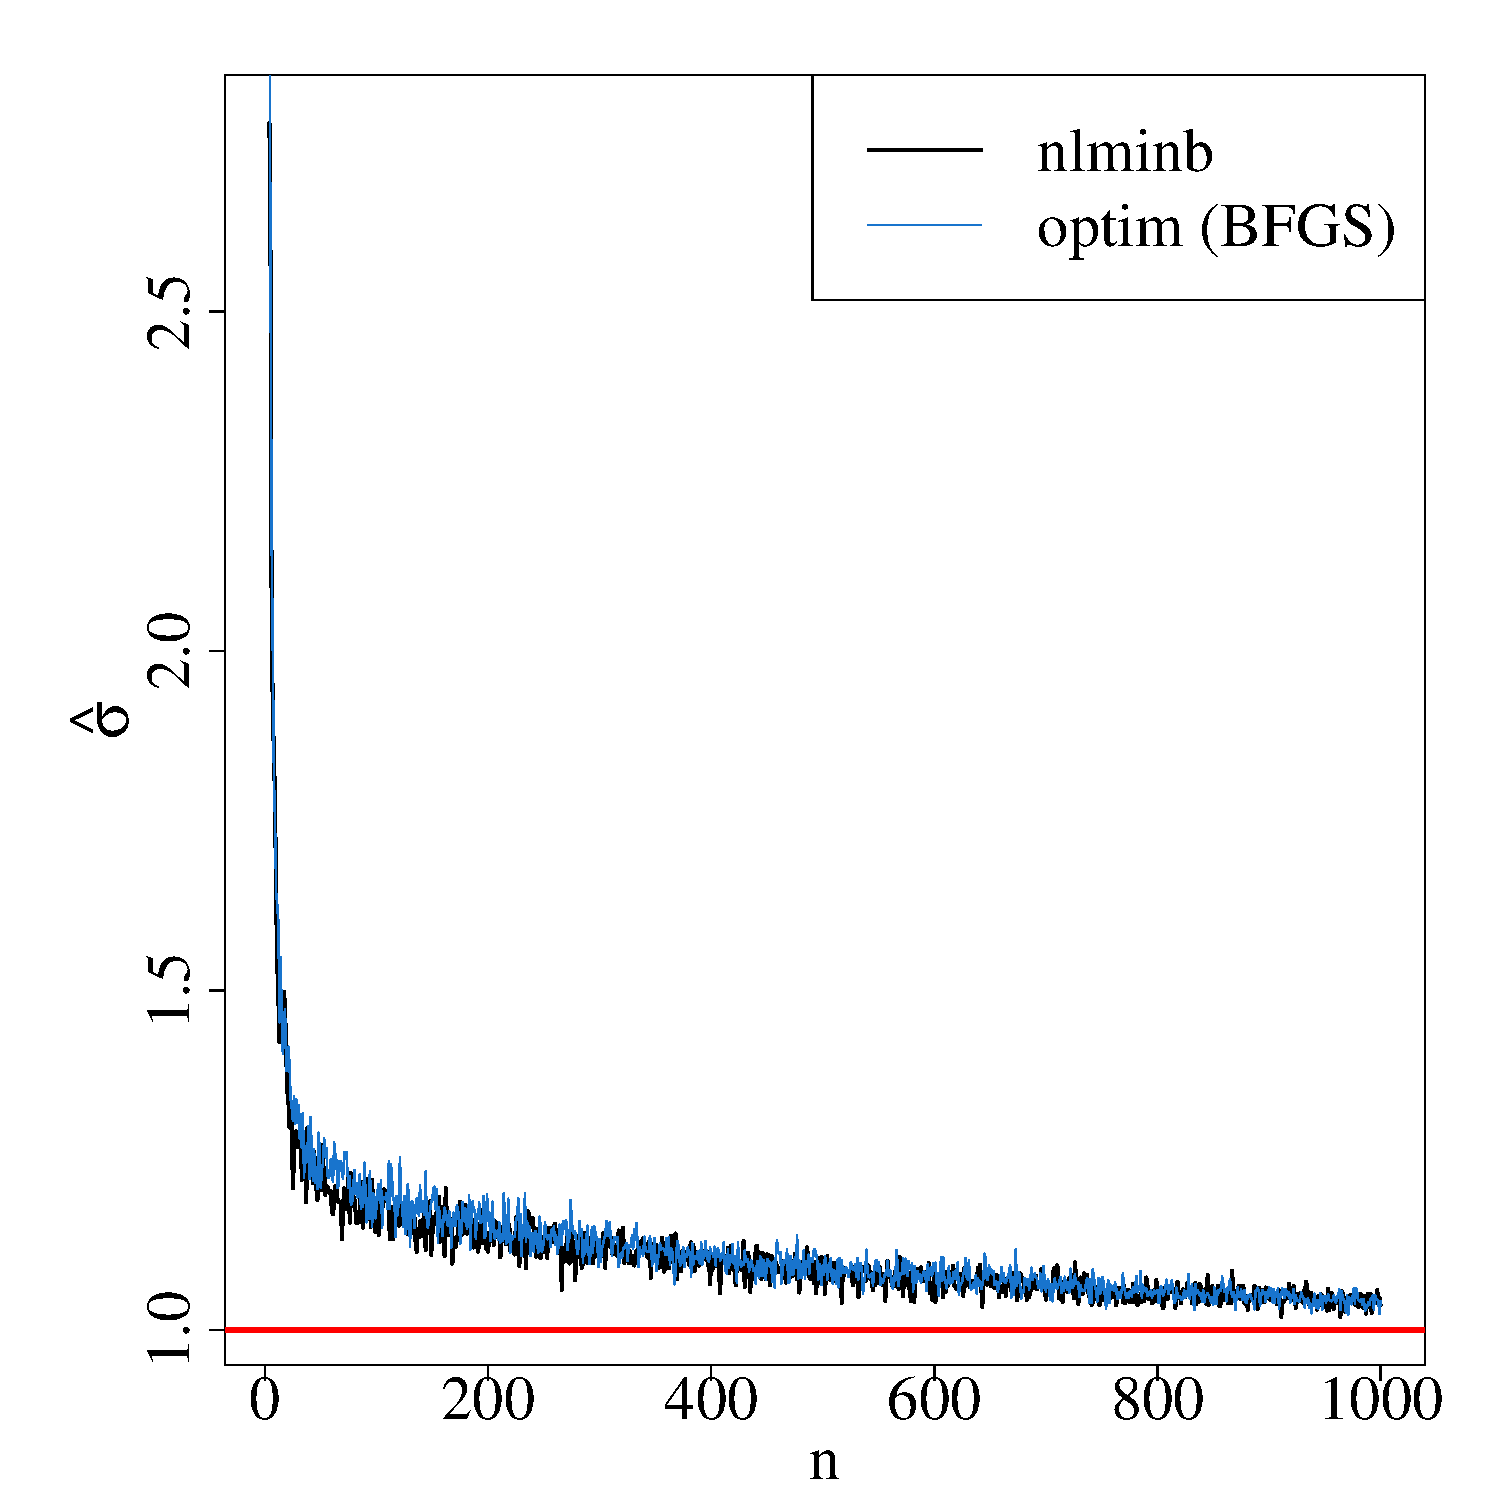
\includegraphics[width=\textwidth]{article-EEBb}
        \caption{\label{fig:EEBb}}
    \end{subfigure}
    ~
    \begin{subfigure}[h]{0.49\textwidth}
        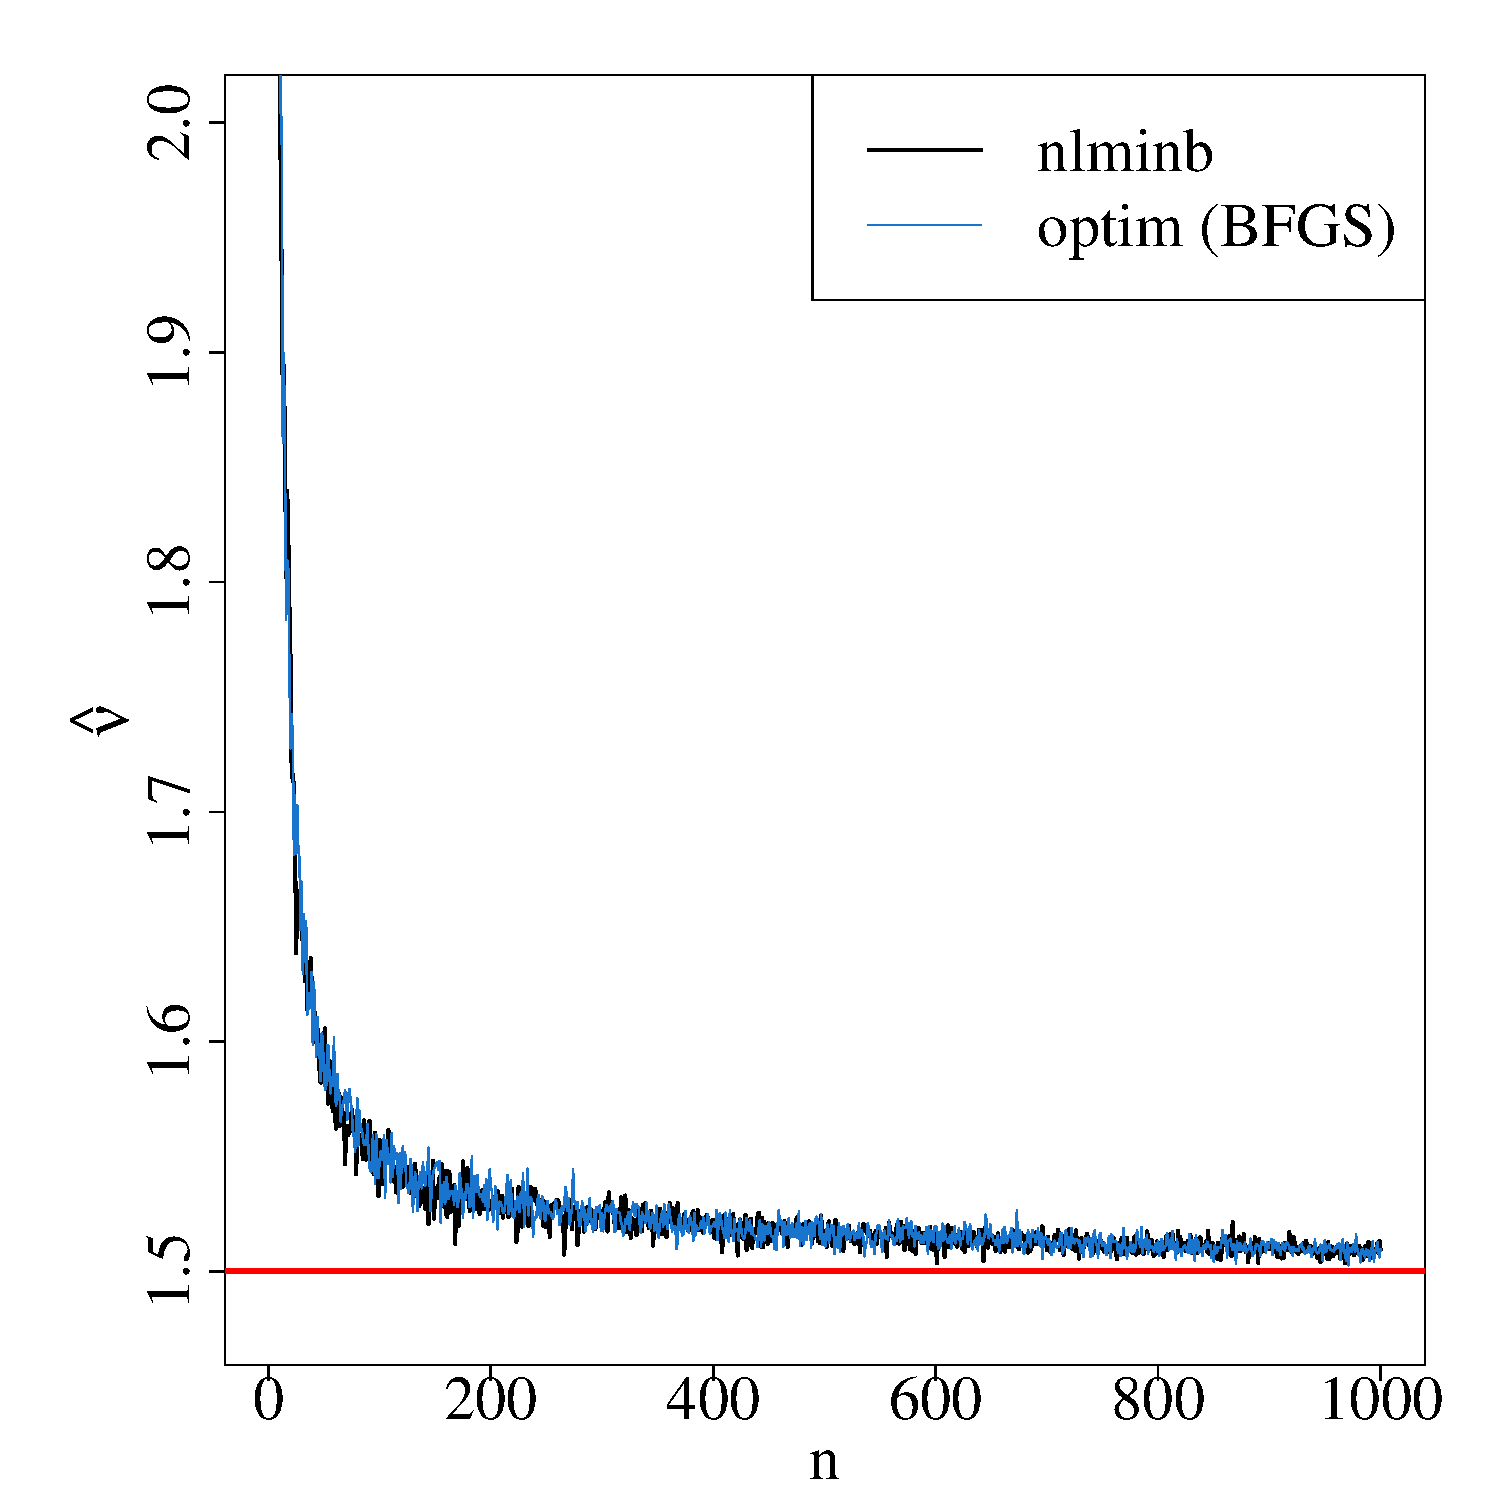
\includegraphics[width=\textwidth]{article-EEBc}
        \caption{\label{fig:EEBc}}
    \end{subfigure}
\caption{\label{fig:EEB} Mean value for (a) proportion of successes $\hat{\mu}$, (b) scale parameter $\hat{\sigma}$ and (c) shape parameter $\hat{\tau}$ versus sample size $n$ in EEB distribution based on 1000 replications. Horizontal red lines are the true value of the parameters.}
\vspace{1.5cm}
\end{figure}

Variance of estimated parameters decreases as sample size increases, according to the efficiency property of ML estimators \citep{Gurland1954, Daniels1961}. This results are presented in figures \ref{fig:varnorm}, \ref{fig:varZIP} and \ref{fig:varEEB} of Appendix \ref{append:variance}.



\begin{figure}[H]
  \centering
    \begin{subfigure}[h]{0.49\textwidth}
        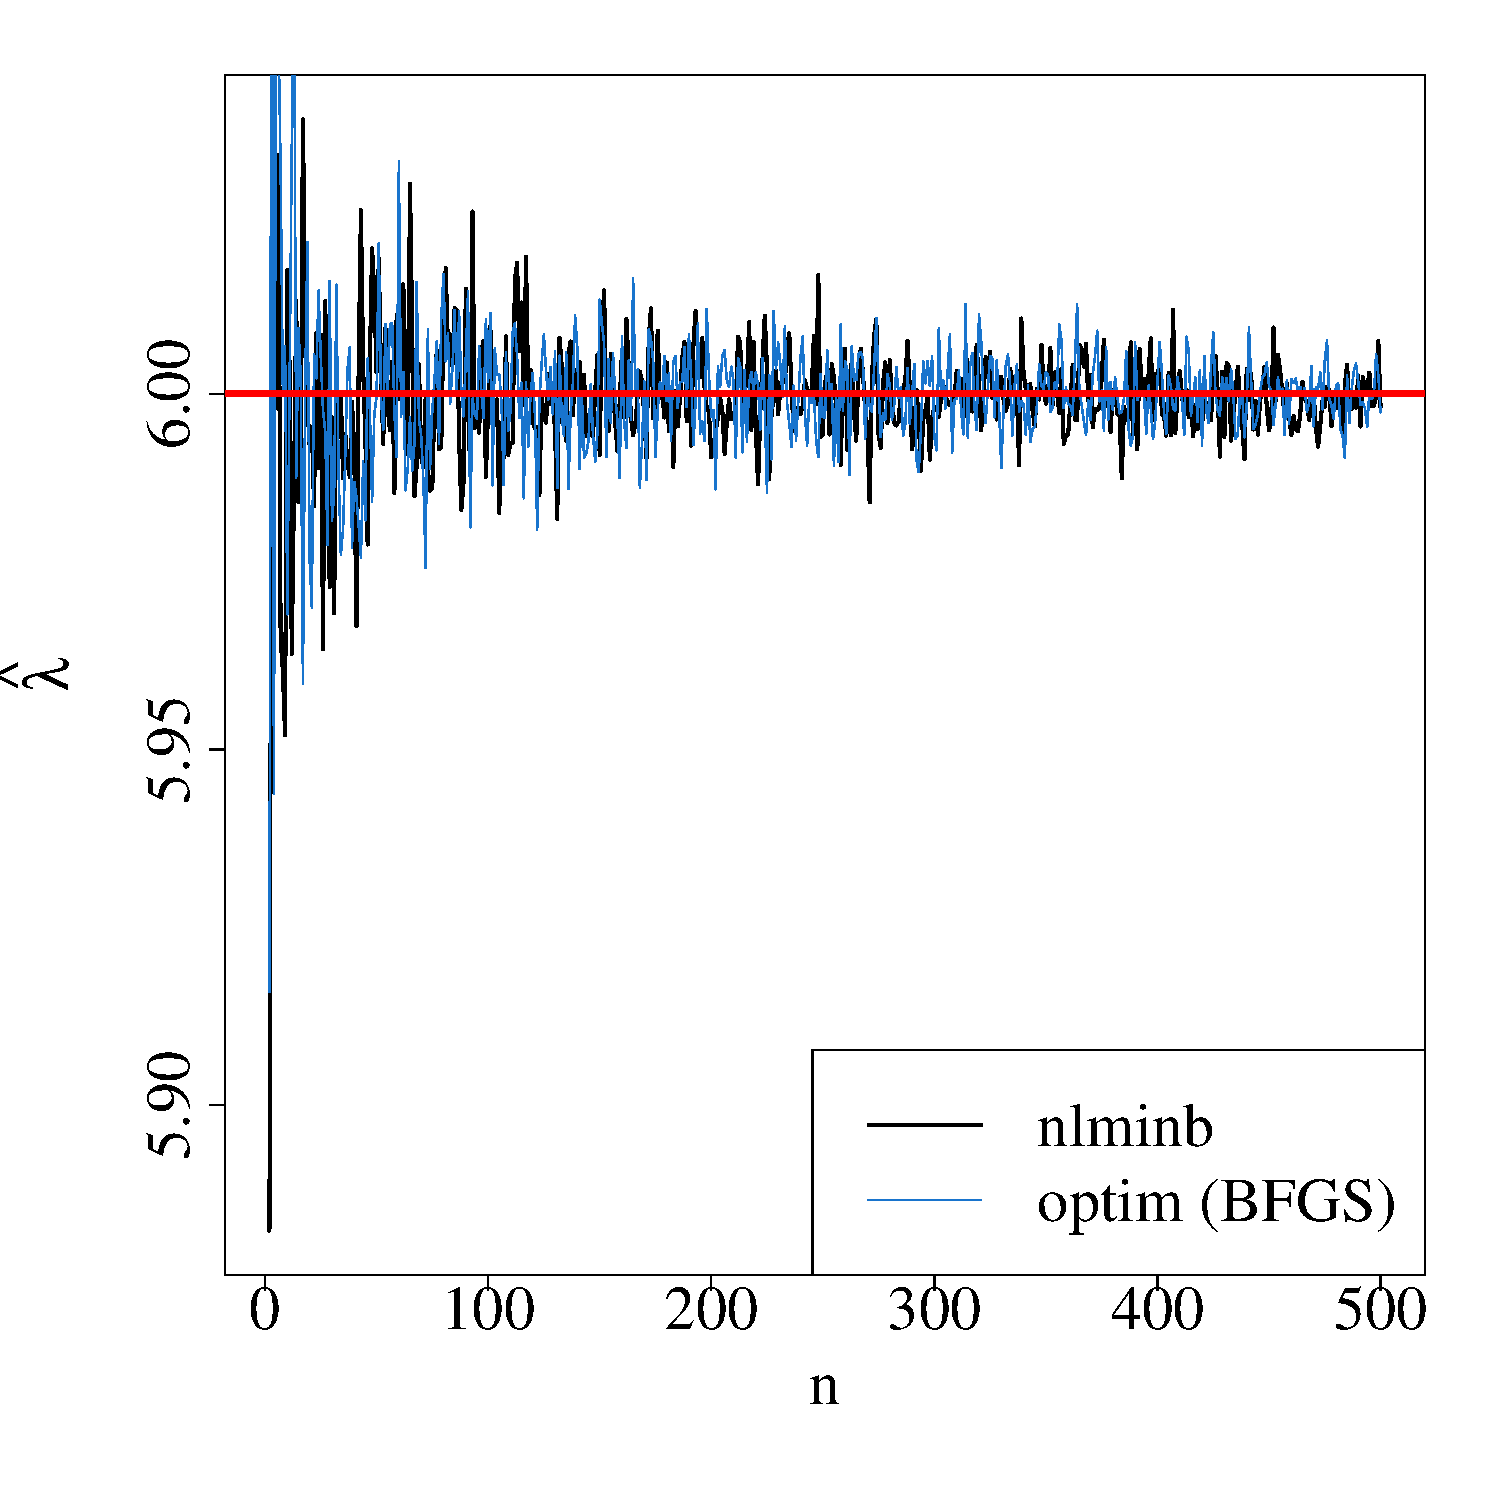
\includegraphics[width=\textwidth]{article-ZIPa}
        \caption{\label{fig:ZIPa}}
    \end{subfigure}
    \begin{subfigure}[h]{0.49\textwidth}
        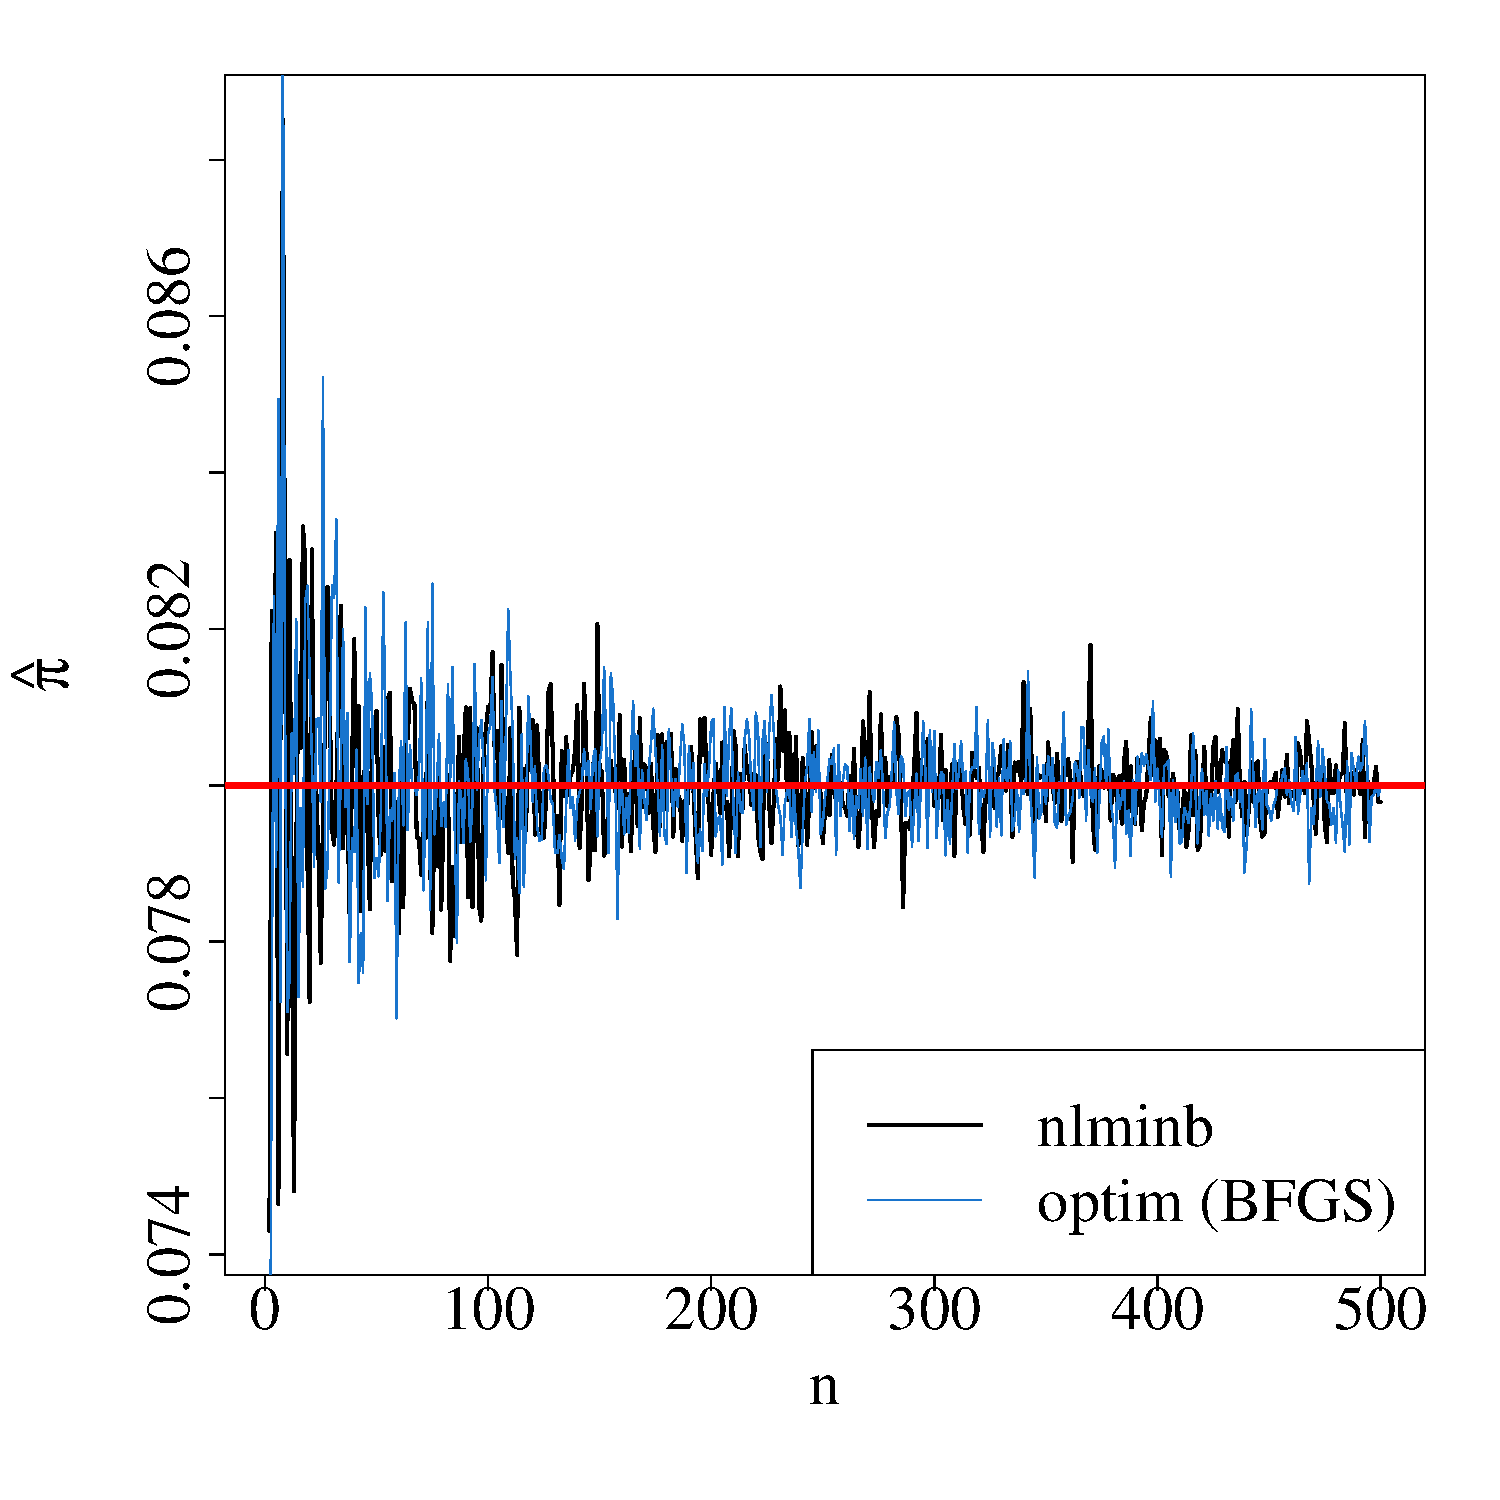
\includegraphics[width=\textwidth]{article-ZIPb}
        \caption{\label{fig:ZIPb}}
    \end{subfigure}
\caption{\label{fig:ZIP} Mean value for (a) rate parameter $\hat{\lambda}$ and (b) extra zeros proportion $\hat{\pi}$ versus sample size $n$ in ZIP distribution based on 1000 replications. Horizontal red lines are the true value of the parameters.}
\end{figure}

%% -- Illustrations ------------------------------------------------------------

%% - Virtually all JSS manuscripts list source code along with the generated
%%   output. The style files provide dedicated environments for this.
%% - In R, the environments {Sinput} and {Soutput} - as produced by Sweave() or
%%   or knitr using the render_sweave() hook - are used (without the need to
%%   load Sweave.sty).
%% - Equivalently, {CodeInput} and {CodeOutput} can be used.
%% - The code input should use "the usual" command prompt in the respective
%%   software system.
%% - For R code, the prompt "R> " should be used with "+  " as the
%%   continuation prompt.
%% - Comments within the code chunks should be avoided - these should be made
%%   within the regular LaTeX text.

\section{Illustrative examples} \label{sec:illustrations}

In the following examples we replicate maximum likelihood method with \code{maxlogL} in two applications: fitting of a power Lindley distribution to model tensile strength of carbon fibers and parameter estimation in two stage hierarchical model of retention proportions in memory tests.

\subsection{Tensile strength data: power Lindley distribution}

\begin{table}[H]
\centering
\begin{tabular}{lllllllllll}
      &       &       &       &       &       &       &       &       &       &       \\ \hline
1.312 & 1.314 & 1.479 & 1.552 & 1.700 & 1.803 & 1.861 & 1.865 & 1.944 & 1.958 & 1.966 \\
1.997 & 2.006 & 2.027 & 2.055 & 2.063 & 2.098 & 2.14  & 2.179 & 2.224 & 2.240 & 2.253 \\
2.270 & 2.272 & 2.274 & 2.301 & 2.301 & 2.359 & 2.382 & 2.382 & 2.426 & 2.434 & 2.435 \\
2.478 & 2.490 & 2.511 & 2.514 & 2.535 & 2.554 & 2.566 & 2.57  & 2.586 & 2.629 & 2.633 \\
2.642 & 2.648 & 2.684 & 2.697 & 2.726 & 2.770 & 2.773 & 2.800 & 2.809 & 2.818 & 2.821 \\
2.848 & 2.88  & 2.954 & 3.012 & 3.067 & 3.084 & 3.090 & 3.096 & 3.128 & 3.233 & 3.433 \\
3.585 & 3.585 &       &       &       &       &       &       &       &       &       \\ \hline
\end{tabular}
\caption{\label{tab:PLdata}Tensile strength of 69 fibers \citep{Devendra2013}.}
\end{table}

Data presented in Table \ref{tab:PLdata} correspond to the tensile strength $T$ (in GPa) of 69 specimens of carbon fiber tested under tension at gauge lengths of 20 mm.

\cite{Ghitany2013} fitted their power Lindley (PL) distribution:

\begin{equation}
f(u|\mu,\sigma) = \frac{\mu \sigma^2}{\sigma + 1} (1 + u^\mu) u ^ {\mu - 1} e^{-\sigma u ^\mu}, \quad u>0, \: \mu, \sigma>0.
\end{equation}

We implemented this density function in the \proglang{R} function \code{dPL} displayed below:

\begin{Schunk}
\begin{Sinput}
R> dPL <- function(x, mu, sigma, log=FALSE){
+    if (any(x < 0))
+      stop(paste("x must be positive", "\n", ""))
+    if (any(mu <= 0))
+      stop(paste("mu must be positive", "\n", ""))
+    if (any(sigma <= 0))
+      stop(paste("sigma must be positive", "\n", ""))
+  
+    loglik <- log(mu) + 2*log(sigma) - log(sigma+1) +
+      log(1+(x^mu)) + (mu-1)*log(x) - sigma*(x^mu)
+  
+    if (log == FALSE)
+      density <- exp(loglik)
+    else density <- loglik
+    return(density)
+  }
\end{Sinput}
\end{Schunk}

Then, we estimate parameters with \code{maxlogL} taking the vector of strengths from data set \code{fibers}, as follows:

\begin{Schunk}
\begin{Sinput}
R> # Fitting of tensile strenght data
R> st <- Fibers$Strenght
R> theta <- maxlogL(x = st, dist = "dPL",
+                   link = list(over = c("mu", "sigma"),
+                               fun = c("log_link", "log_link")))
R> summary(theta)
\end{Sinput}
\begin{Soutput}
---------------------------------------------------------------
Optimization routine: nlminb 
Standard Error calculation: Hessian from optim 
---------------------------------------------------------------
      AIC    BIC
  102.119 98.119
---------------------------------------------------------------
      Estimate  Std. Error
mu     3.867777     0.3137
sigma  0.049671     0.0160
-----
\end{Soutput}
\end{Schunk}

Estimations are $\hat{\mu}=3.8678$ and $\hat{\sigma}=0.0497$. Essentially, we get the same values computed by \cite{Ghitany2013}. In Figure \ref{fig:PL} we showed the performance of parameter estimation plotting corresponding density along with the histogram in the left panel and estimated survival function along with Kaplan-Meier estimator in the right panel.



\begin{figure}[H]
\centering
    \begin{subfigure}[h]{0.49\textwidth}
        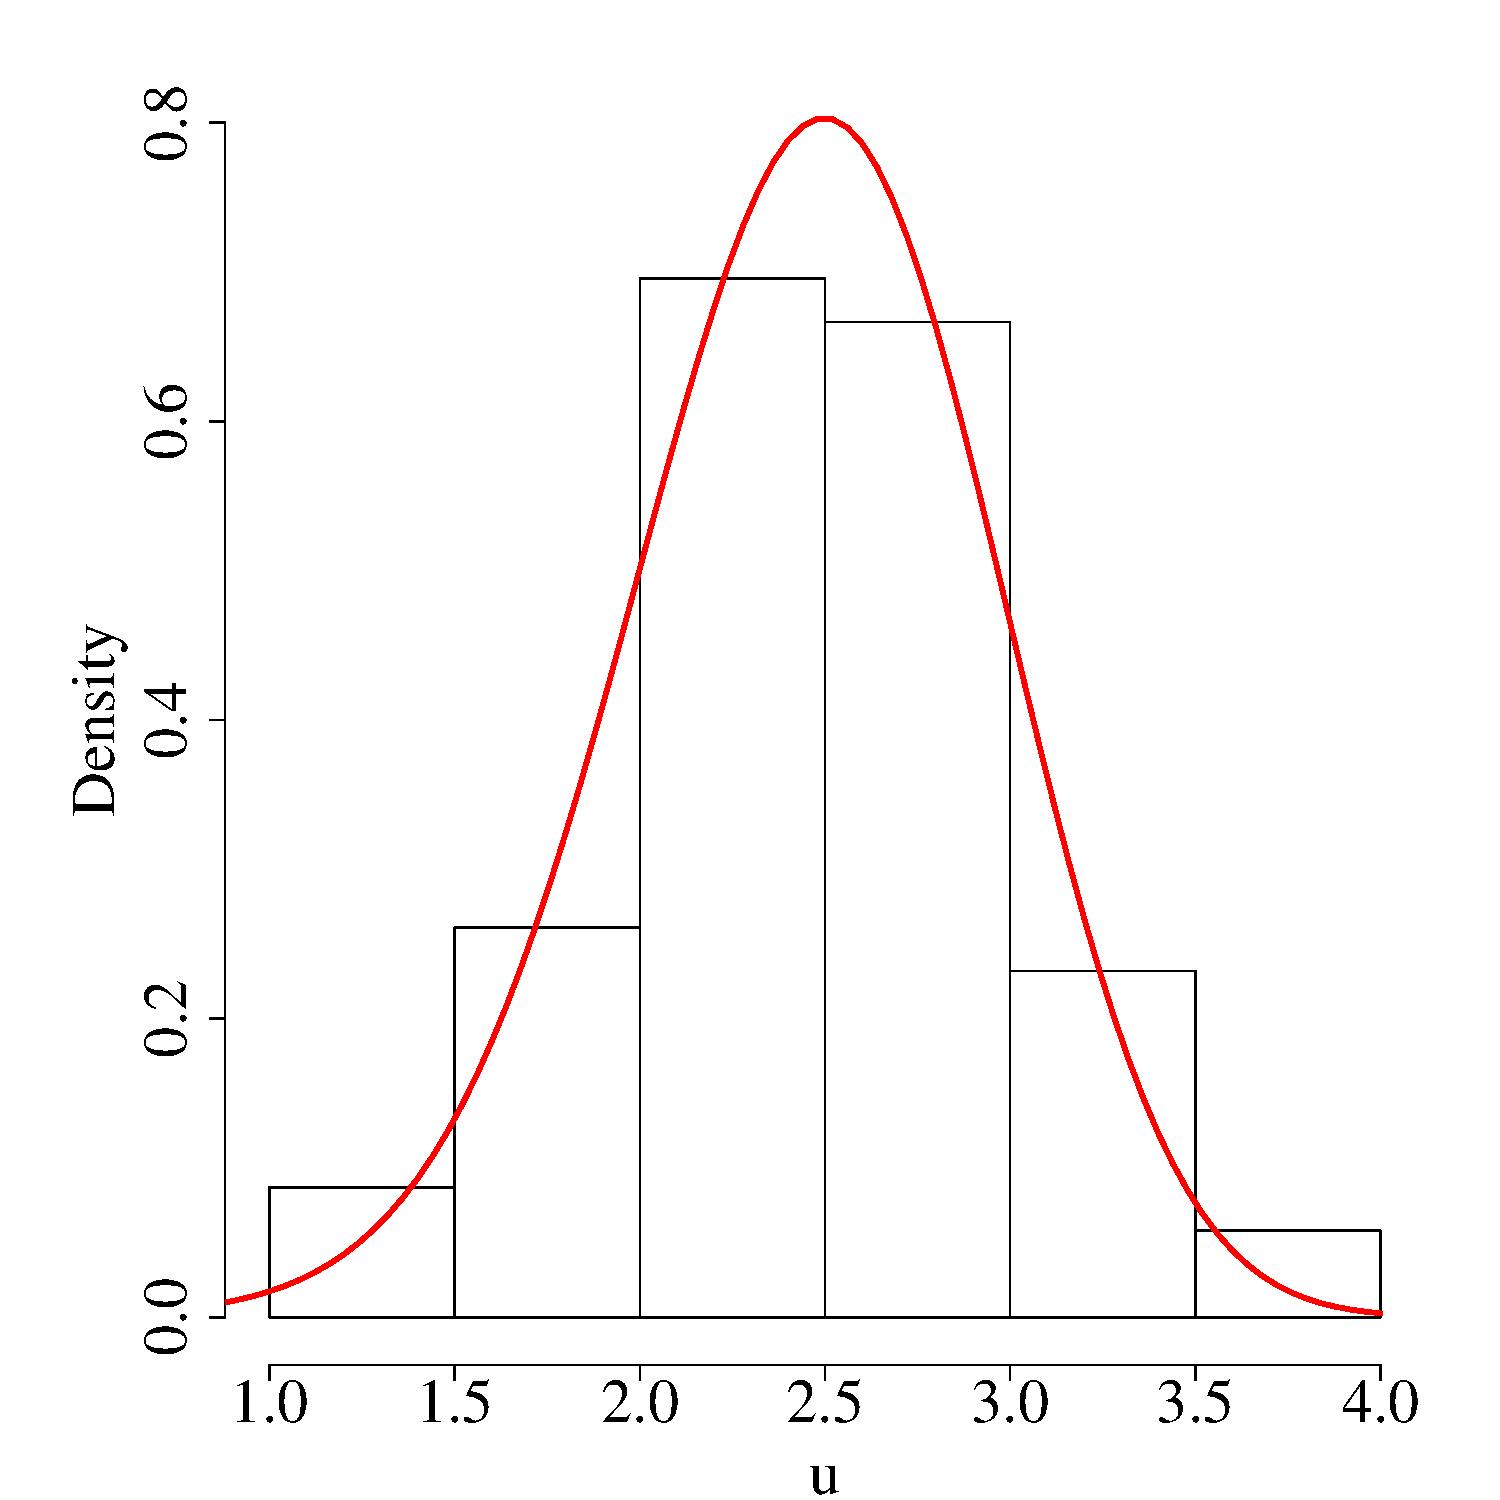
\includegraphics[width=\textwidth]{article-PLexample_a}
        \caption{\label{fig:density}}
    \end{subfigure}
    \begin{subfigure}[h]{0.49\textwidth}
        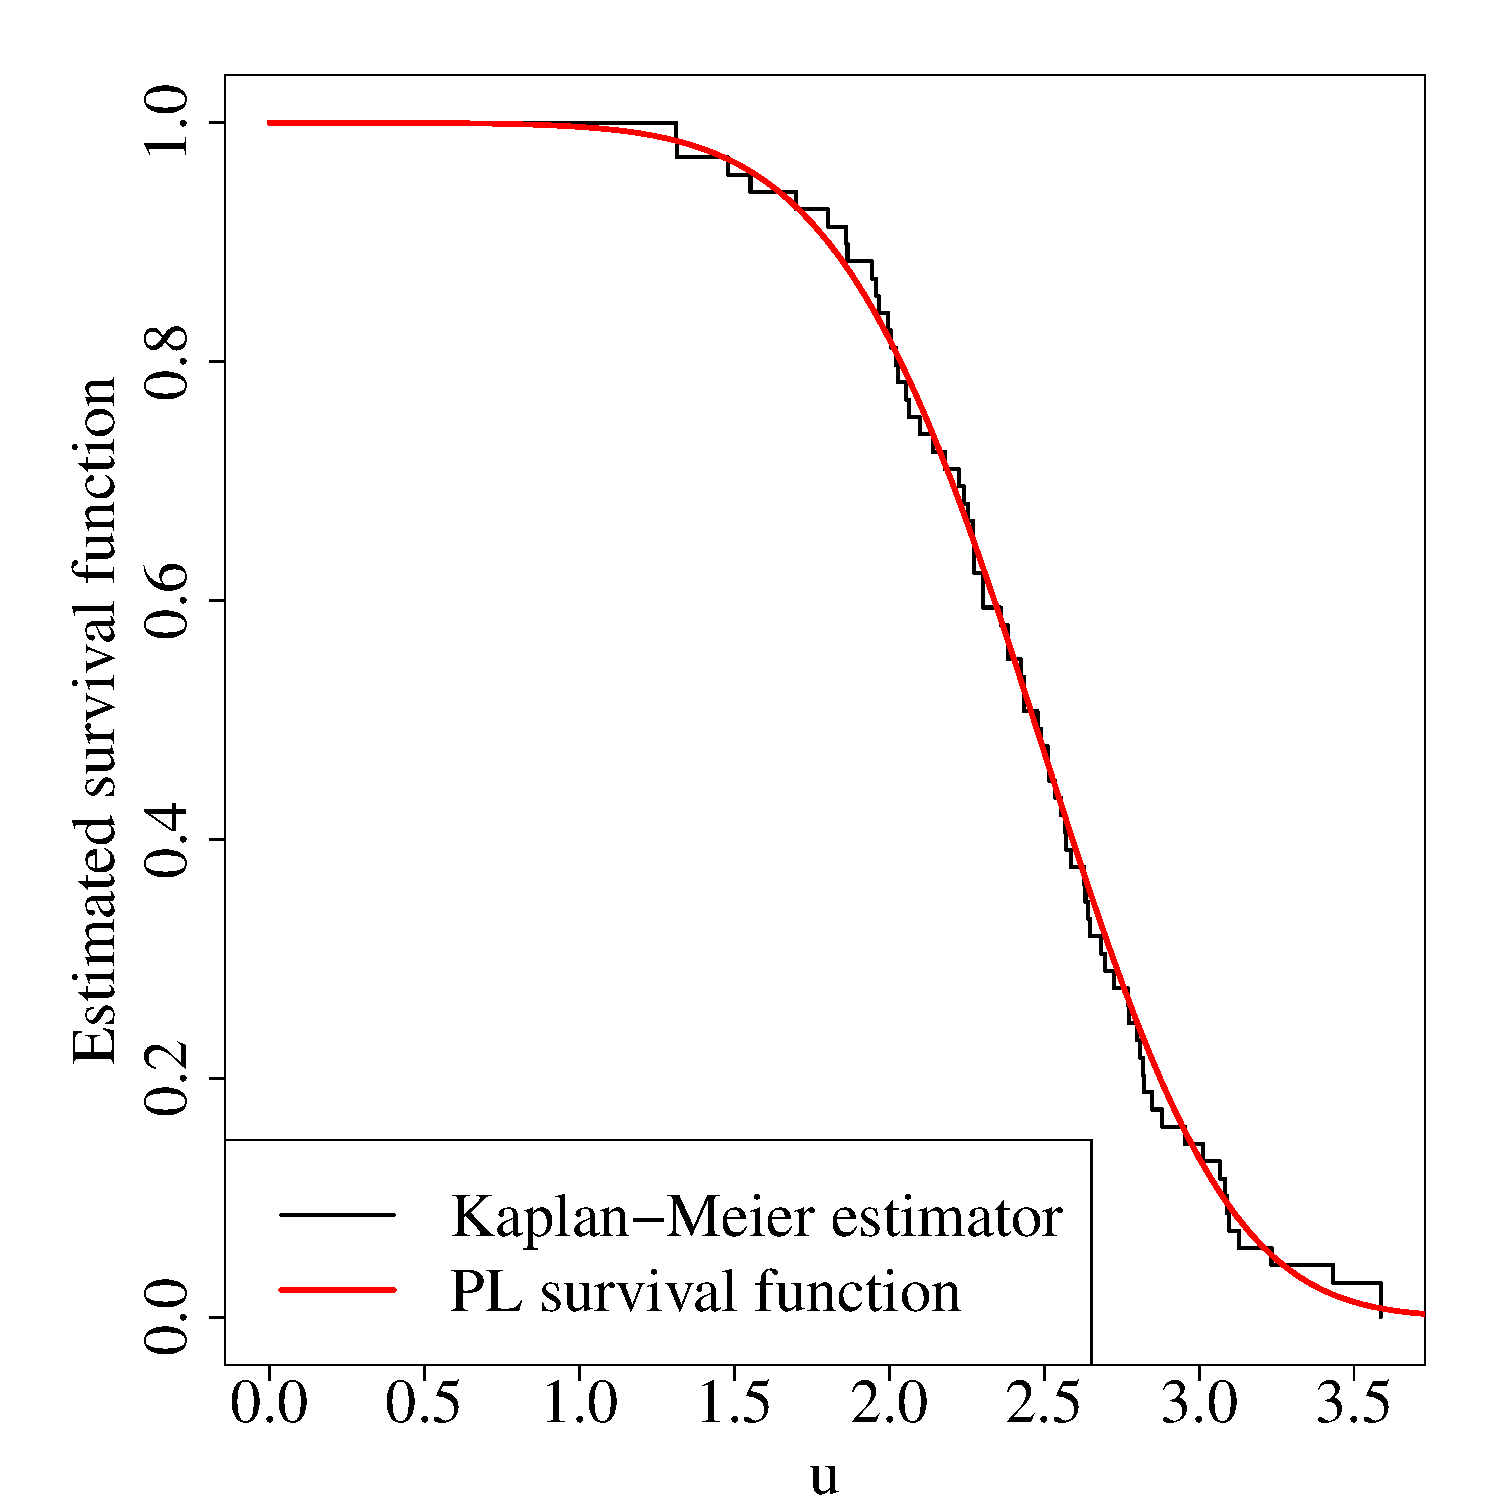
\includegraphics[width=\textwidth]{article-PLexample_b}
        \caption{\label{fig:survival}}
    \end{subfigure}
\caption{\label{fig:PL} Fitting of tensile strength data: (a) estimated density and histogram; (b) estimated power Lindley survival function and Kaplan-Meier estimator.}
\end{figure}

\subsection{Forgetting data: hierarchical binomial distribution}

\code{maxlogL} is capable of fit hierarchical models with the proper function definition of input variable. To illustrate the estimation, we replicated forgetting data example presented in \cite{Myung2003}, which used data from \cite{MurdockBennetB.1961}.

The retention function is a probability function that models the proportion of correct recall at time $t_i$ in each trial in memory tests. \cite{Myung2003} studied the following two models in their application example:

\begin{equation}\label{priors}
  \begin{split}
    \text{power model: }p(a, b, t) & = at^{-b}, \\
    \text{exponential model: }p(a, b, t) & = ae^{-b t}, \quad a, b > 0.
  \end{split}
\end{equation}

\begin{table}[h!]
\centering
\begin{tabular}{|l|cccccc|}
\hline
\multicolumn{7}{|c|}{$m=100$ (number of trials)}                      \\ \hline
Retention Interval (sec.) & 1    & 3    & 6    & 9    & 12   & 18   \\ \hline
Observed proportion       & 0.94 & 0.77 & 0.40 & 0.26 & 0.24 & 0.16 \\ \hline
\end{tabular}
\caption{Observed proportion of recalls at each time.}
\end{table}

Each observation in the data set corresponds to a proportion obtained as the quotient of correct responses ($x_i$) and the total number of independent trials (replications of each memory test, represented by $m$). This kind of experiment can be modeled with a binomial distribution:

\begin{equation} \label{posterior}
  f(x_i|a, b, m) = \frac{m!}{(m-x_i)!\: x_i!}p(a, b, t_i) \left[ 1-p(a, b, t_i) \right]^{m-x_i}
\end{equation}

The usefulness of each retention equation is given by their goodness of fit.

\subsection*{Power model implementation}

The hierarchical model with power retention function is implemented in an \proglang{R} function as follows:

\begin{Schunk}
\begin{Sinput}
R> # Power model implementation
R> power_logL <- function(x, a, b, log = FALSE){
+    p <- a * x[,1]^(-b)
+    f <- dbinom(x = x[,2], size = m, prob = p)
+    if (log == TRUE)
+      density <- log(f) else density <- f
+    return(density)
+  }
\end{Sinput}
\end{Schunk}

Conditional density in equation (\ref{posterior}) depends on $x_i$, but proportion of successes depends on $t$, as equation (\ref{priors}) shows. For this reason, the input argument \code{x} must be a $n\times 2$ matrix, where $n$ is the sample size. In forgetting data, $n=6$. Then, the estimation is performed as usual with \code{maxlogL}. Note line six in the following chunk of code, which corresponds to the matrix definition of the input data aforementioned:

\begin{Schunk}
\begin{Sinput}
R> # Power model estimation
R> m <- 100 # Independent trials
R> t <- c(1,3,6,9,12,18) # time intervals
R> p.ob <- c(0.94,0.77,0.40,0.26,0.24,0.16) # Observed proportion
R> x <- p.ob*m # Correct responses
R> x <- as.integer(x)
R> Xi <- matrix(c(t,x), ncol=2, nrow=6)
R> retention.pwr <- maxlogL(x = Xi, dist = "power_logL", lower = c(0.01,0.01),
+                           upper = c(1,1), start = c(0.1,0.1))
R> summary(retention.pwr)
\end{Sinput}
\begin{Soutput}
---------------------------------------------------------------
Optimization routine: nlminb 
Standard Error calculation: Hessian from optim 
---------------------------------------------------------------
      AIC     BIC
  57.4522 53.4522
---------------------------------------------------------------
  Estimate  Std. Error
a   0.95312     0.0186
b   0.49793     0.0324
-----
\end{Soutput}
\end{Schunk}

In this application, convergence was achieved by solving a box-constrained likelihood optimization, whose boundaries were specified in arguments \code{lower} and \code{upper}. Furthermore, tuning initial values was necessary with argument \code{start}. Computed values are $\hat{\boldsymbol{\theta}}=(\hat{a}_{\text{pwr}},\hat{b}_{\text{pwr}})=(0.953,0.498)$, which are the same estimates of \cite{Myung2003}. Power fitting is illustrated in Figure \ref{fig:forgetting}.

\subsection*{Exponential model implementation}

Similarly as before, exponential retention function is implemented and input data is defined as a matrix, in this fashion:

\begin{Schunk}
\begin{Sinput}
R> # Exponential model implementation
R> exp_logL <- function(x, a, b, log = FALSE){
+    p <- a * exp(-x[,1]*b)
+    f <- dbinom(x = x[,2], size = m, prob = p)
+    if (log == TRUE)
+      density <- log(f) else density <- f
+    return(density)
+  }
R> # Exponential model estimation
R> m <- 100 # Independent trials
R> t <- c(1,3,6,9,12,18) # time intervals
R> p.ob <- c(0.94,0.77,0.40,0.26,0.24,0.16) # Observed proportion
R> x <- p.ob*m # Correct responses
R> x <- as.integer(x)
R> Xi <- matrix(c(t,x), ncol=2, nrow=6)
R> retention.exp <- maxlogL(x = Xi, dist = 'exp_logL', lower = c(0.1,0.1),
+                           upper = c(2,2), start = c(0.1,0.2))
R> summary(retention.exp)
\end{Sinput}
\begin{Soutput}
---------------------------------------------------------------
Optimization routine: nlminb 
Standard Error calculation: Hessian from optim 
---------------------------------------------------------------
      AIC     BIC
  41.3329 37.3329
---------------------------------------------------------------
  Estimate  Std. Error
a   1.07011     0.0313
b   0.13083     0.0093
-----
\end{Soutput}
\end{Schunk}

Again, we obtain the same estimates of \cite{Myung2003}: $\hat{\boldsymbol{\theta}}=(\hat{a}_{\text{exp}},\hat{b}_{\text{exp}})=(1.070,0.131)$. Exponential fitting is shown in Figure \ref{fig:forgetting}. According to the Akaike information criterion, the exponential model has better fitness ($AIC_{\text{exp}}=41.33$ against $AIC_{\text{pwr}}=57.45$).


\begin{figure}[H]
\centering
  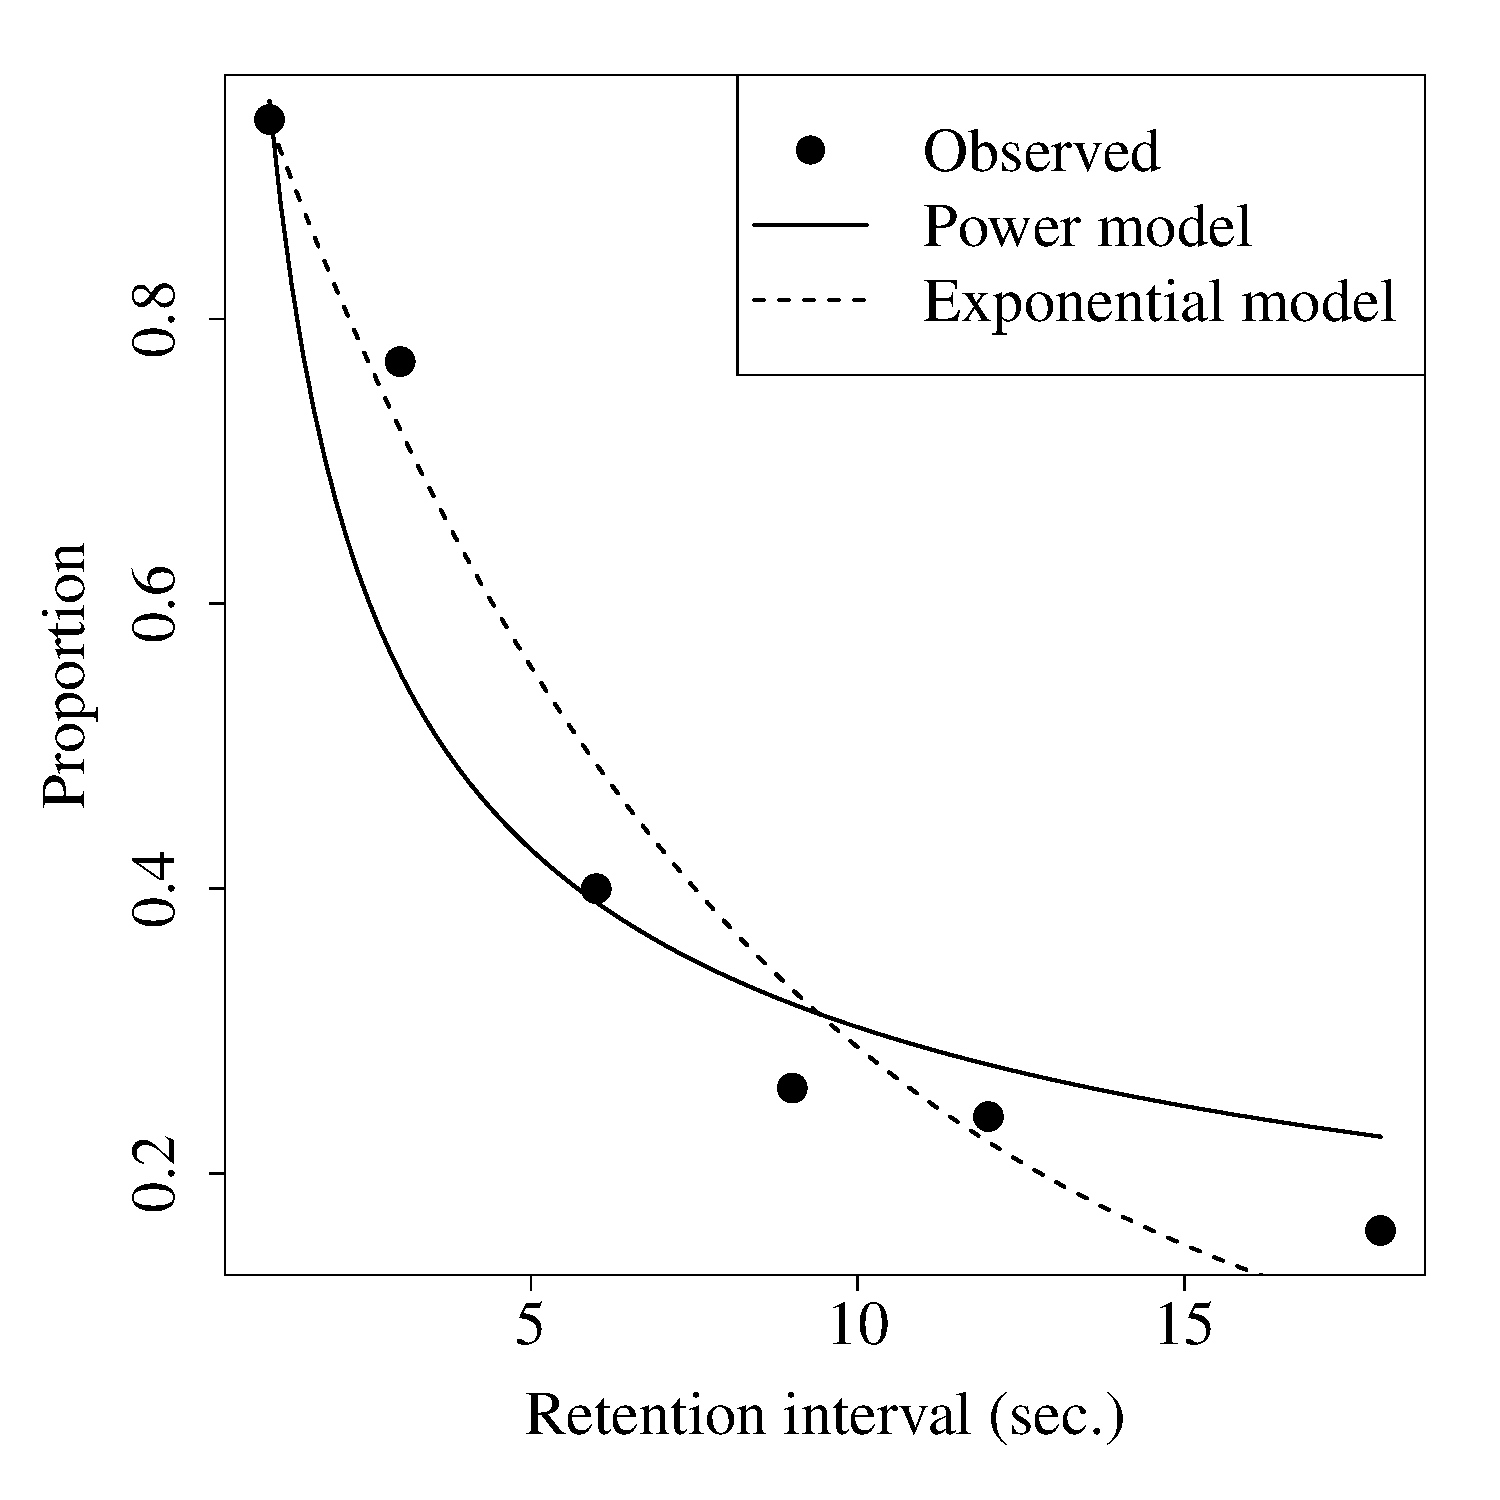
\includegraphics[width=0.6\textwidth]{article-RetentionPlot}
  \caption{\label{fig:forgetting} Observed proportion of recalls and models fitted.}
\end{figure}

% % \section{Aarset data}
% %
% % Data is from Aarset (1987) and they contain the times to failure of 50 devices put on life test
% %
% % \begin{table}[ht]
% % \centering
% % \begin{tabular}{rrrrrrrrrrrrrrrrrrrrrrrrrrrrrrrrrrrrrrrrrrrrrrrrrrrr}
% %   \hline
% % 0.10  & 0.20  & 1.00  & 1.00  & 1.00  & 1.00  & 1.00  & 2.00  & 3.00  & 6.00  & 7.00  \\
% % 1.00  & 1.00  & 12.00 & 18.00 & 18.00 & 18.00 & 18.00 & 18.00 & 21.00 & 32.00 & 36.00 \\
% % 40.00 & 45.00 & 46.00 & 47.00 & 50.00 & 55.00 & 60.00 & 63.00 & 63.00 & 67.00 & 67.00 \\
% % 67.00 & 67.00 & 72.00 & 75.00 & 79.00 & 82.00 & 82.00 & 83.00 & 84.00 & 84.00 & 84.00 \\
% % 85.00 & 85.00 & 85.00 & 85.00 & 85.00 & 86.00 & 86.00 \\
% %    \hline
% % \end{tabular}
% % \caption{\label{tab:Aarset}Failure time of 50 devices.}
% % \end{table}
% %
% % This data has been fitted by Mudholkar and Srivastava, Xie and Lai , Lai et al., Sarhan and Zaindin and Silva et al. Almalki et al. (2013) fitted their NMW distribution via ML estimation. The pdf is as follows
% %
% % \begin{equation}
% % f(t|\alpha, \beta, \gamma, \theta, \lambda) = \left( \alpha\theta t^{\theta-1} + \beta (\gamma+\lambda t)t^{\gamma-1}e^{\lambda t} \right)e^{-\alpha t^\theta -\beta t^\gamma e^{\lambda t}}, \quad t>0
% % \end{equation}
% %
% % In first place, we must implement the corresponding pdf
% %
% % <<echo=TRUE, eval=TRUE>>=
% % dNMW <- function(x, alpha, beta, gamma, theta, lambda, log = FALSE){
% %   if (any(x<0))
% %     stop(paste("x must be positive", "\n", ""))
% %   if (any(alpha<=0 ))
% %     stop(paste("alpha must be positive", "\n", ""))
% %   if (any(beta<=0))
% %     stop(paste("beta must be positive", "\n", ""))
% %   if (any(theta<=0))
% %     stop(paste("theta must be positive", "\n", ""))
% %   if (any(gamma<=0))
% %     stop(paste("gamma must be positive", "\n", ""))
% %   if (any(lambda<0))
% %     stop(paste("lambda must be positive", "\n", ""))
% %
% %   loglik<- log(alpha*theta*(x^(theta-1)) + exp(lambda*x)*beta*(gamma+lambda*x)*x^(gamma-1)) -
% %            alpha*(x^theta) - beta*(x^gamma)*exp(lambda*x)
% %
% %   if (log == FALSE)
% %     density<- exp(loglik)
% %   else
% %     density <- loglik
% %   return(density)
% % }
% % @
% %
% % Then, we implement \code{maxlogL} routine
% %
% % <<warining=FALSE, message=FALSE>>=
% % # res <- maxlogL(x = Aarset, dist = 'dNMW', lower = numeric(5)+1e-10,
% % #                upper = c(0.1,0.001,0.05,1,0.5))
% % # summary(res)
% % @

%% -- Summary/conclusions/discussion -------------------------------------------

\section{Conclusions} \label{sec:conclussions}

We have implemented classic estimation via maximization of log-likelihood function through basic optimization routines in \proglang{R} such as \code{optim} and \code{nlminb}. With \code{maxlogL}, we enable researchers, developers and users in general to compute ML estimators of any distribution in a fast and reliable way. With our \code{summary} method, it ia possible to calculate standard error of estimates through Hessian matrix or bootstrap algortihm. In some cases, it is possible to implement estimation in hierarchical models, with appropriate tunning of initial values. \\

In future revisions, we could implement evolutionary algorithms to perform estimation in distributions with regularity issues \citep{Haupt2003}. Furthermore, our routine could be took to develop further work on log-likelihood estimation, such as developing new parametric regression models.

\bibliography{refs}

%% -- Appendix (if any) --------------------------------------------------------
%% - After the bibliography with page break.
%% - With proper section titles and _not_ just "Appendix".

\newpage

\begin{appendix}

\section{Variance of estimates} \label{append:variance}

In this section we report results of variance versus sample size of ML estimation with distributions fitted with \code{maxlogL} in section \ref{sec:results}.

\subsection{Normal distribution}



\begin{figure}[ht]
    \vspace{-20pt}
    \begin{subfigure}[h]{0.49\textwidth}
        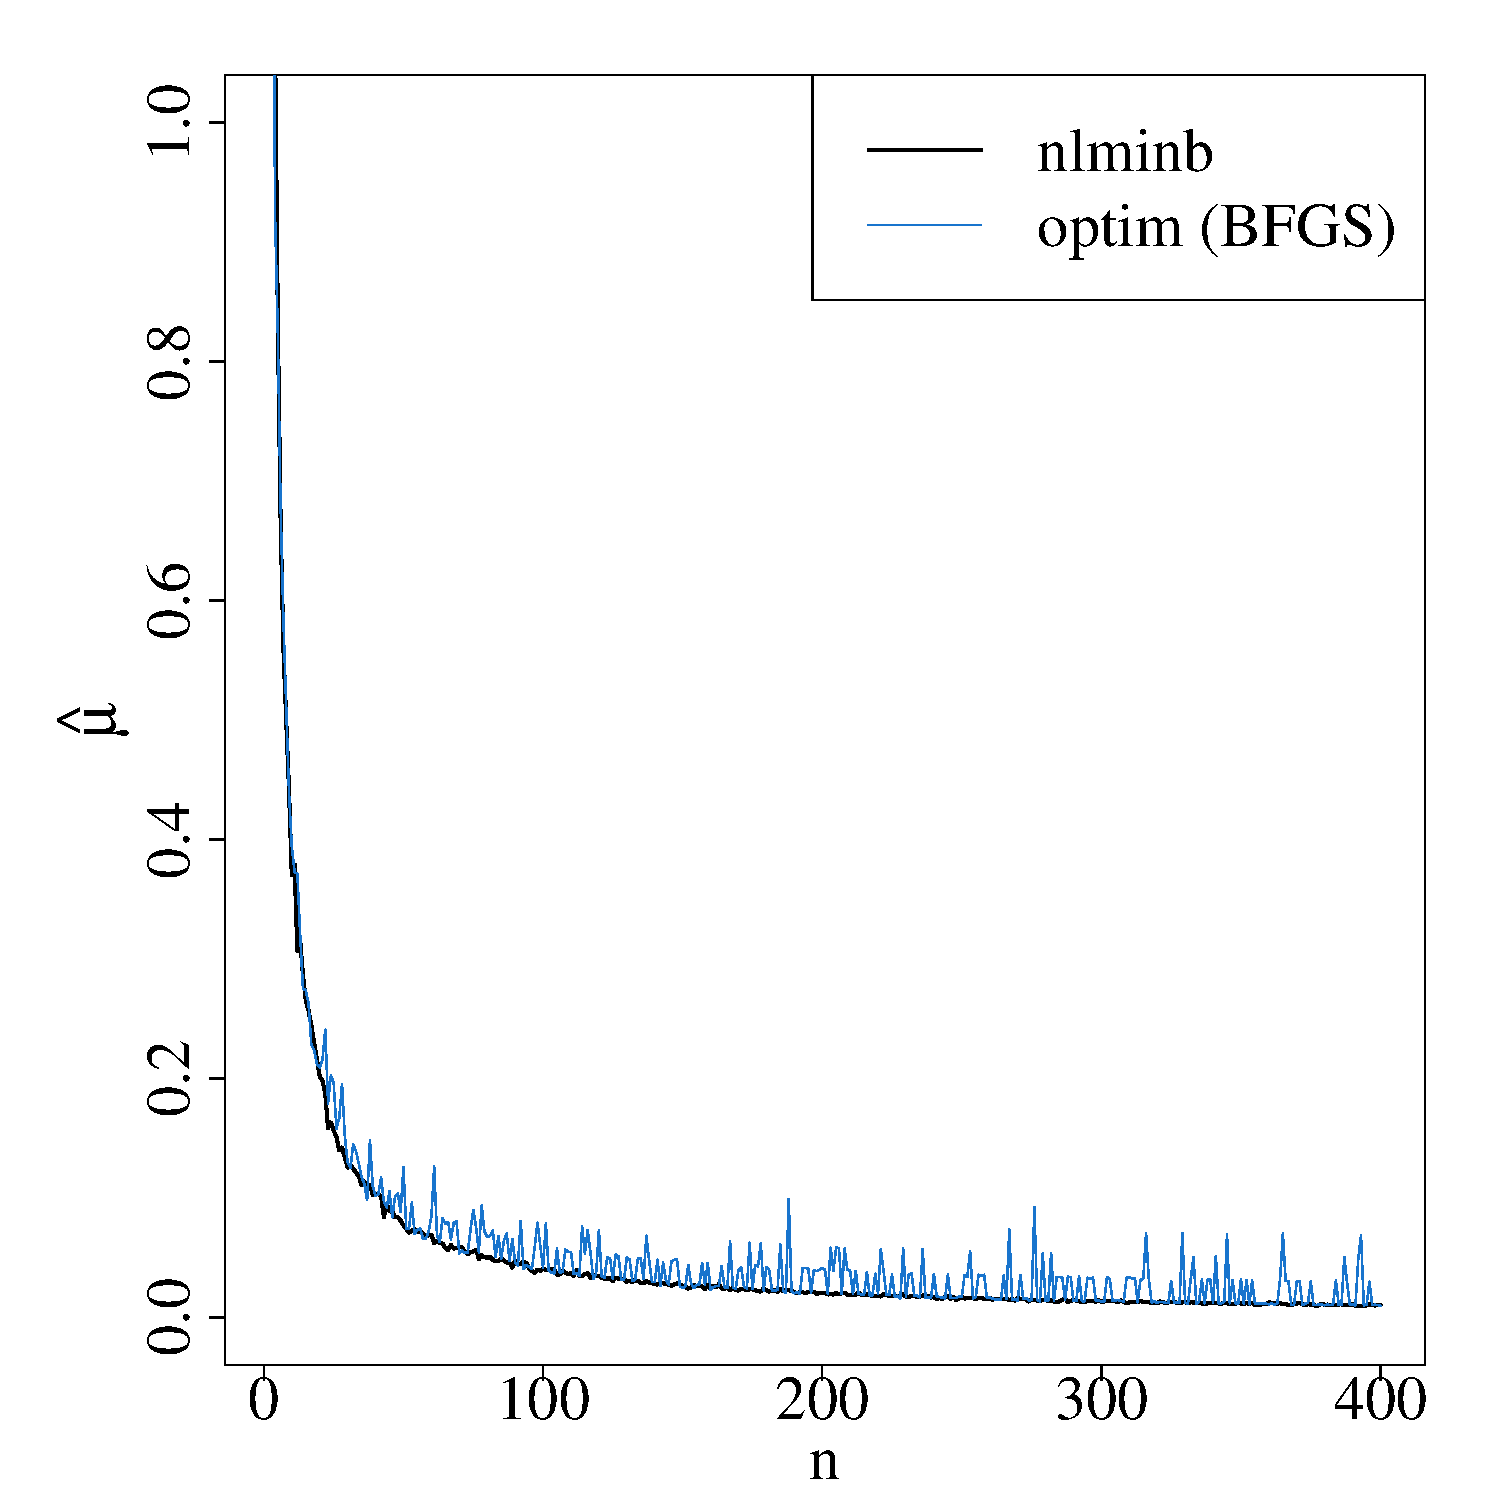
\includegraphics[width=\textwidth]{article-varnorm_a}
        \caption{\label{fig:norma}}
    \end{subfigure}
    \begin{subfigure}[h]{0.49\textwidth}
        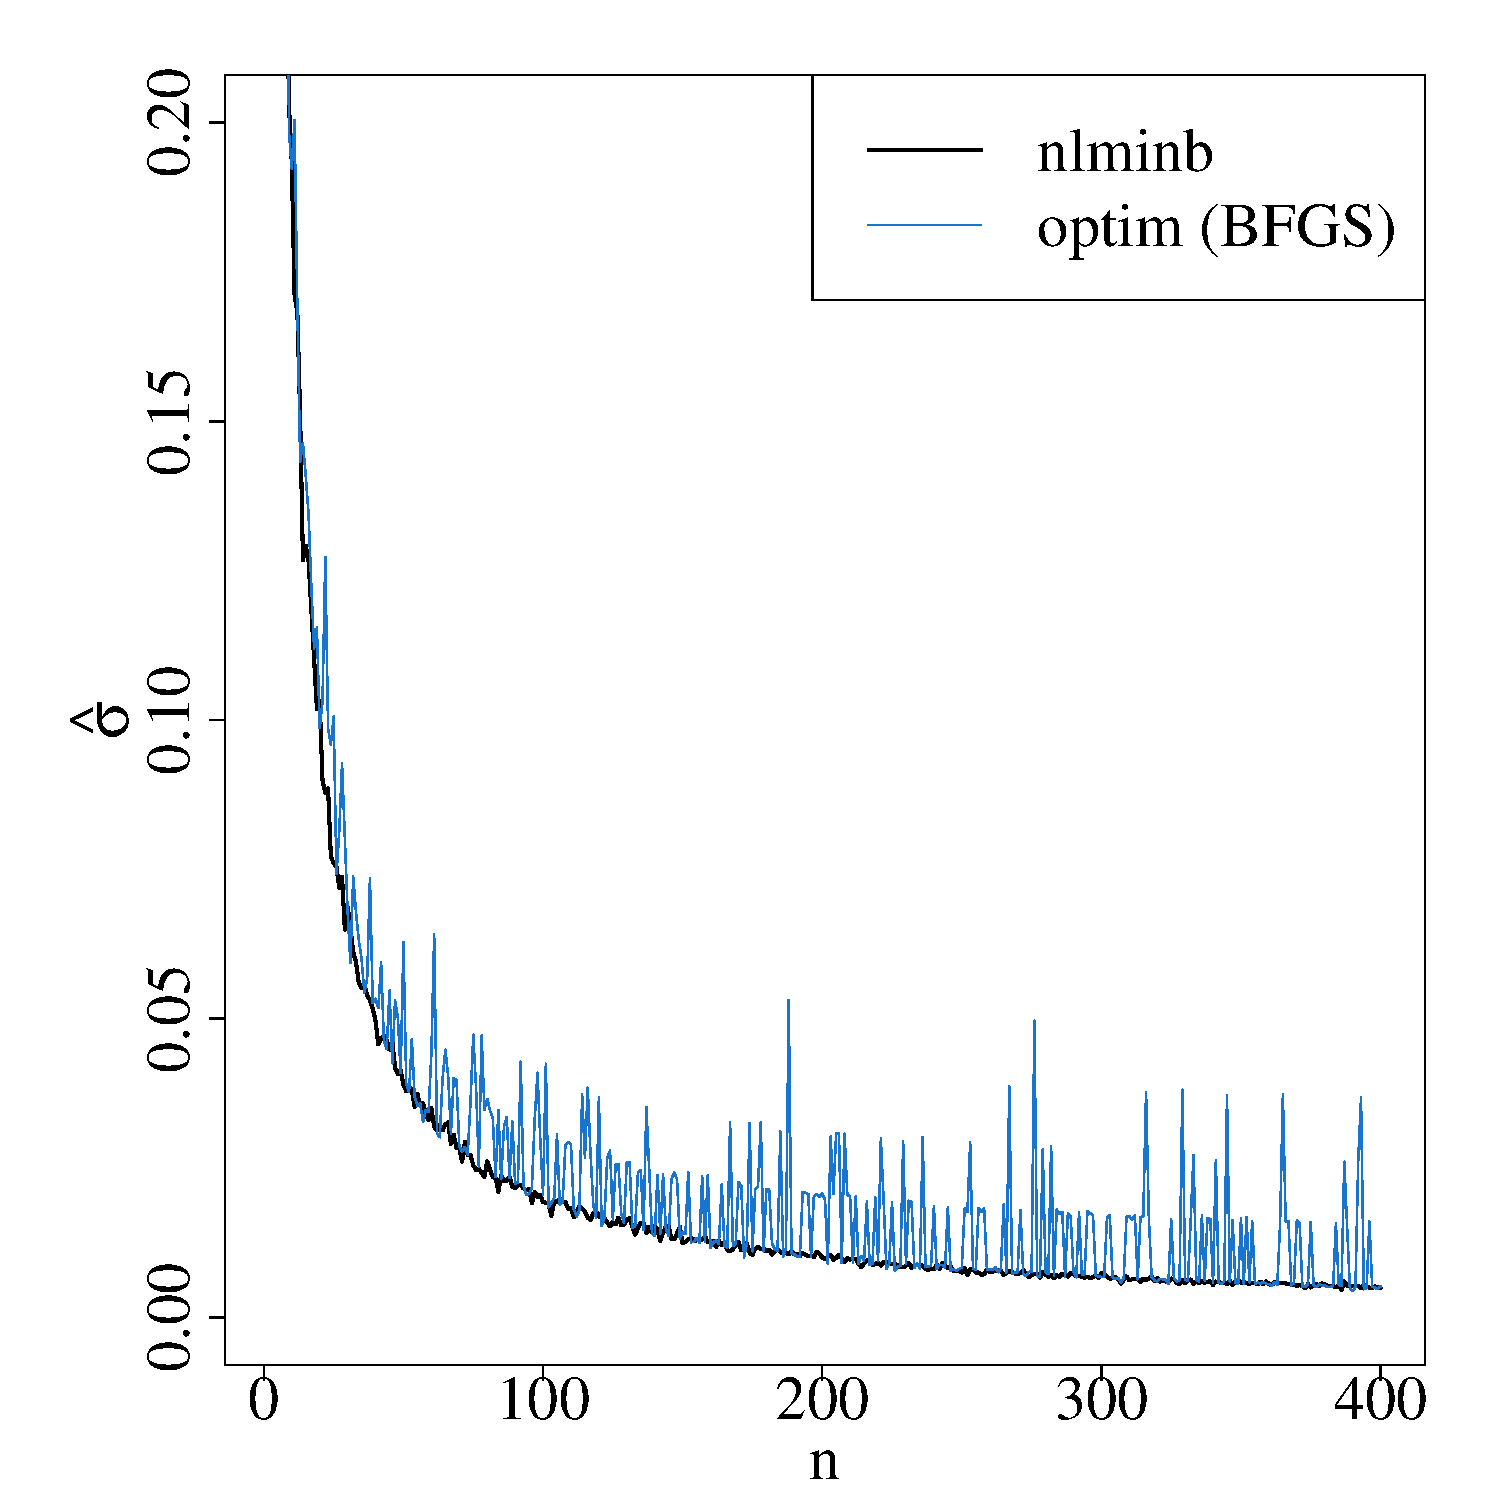
\includegraphics[width=\textwidth]{article-varnorm_b}
        \caption{\label{fig:varnormb}}
    \end{subfigure}
\caption{\label{fig:varnorm}  Variance for (a) location parameter $\hat{\mu}$ and (b) scale parameter $\hat{\sigma}$ versus sample size $n$ in normal distribution based on 1000 replications..}
\vspace{-20pt}
\end{figure}

\subsection{ZIP distribution}



\begin{figure}[h]
  \vspace{-20pt}
  \centering
    \begin{subfigure}[h]{0.49\textwidth}
        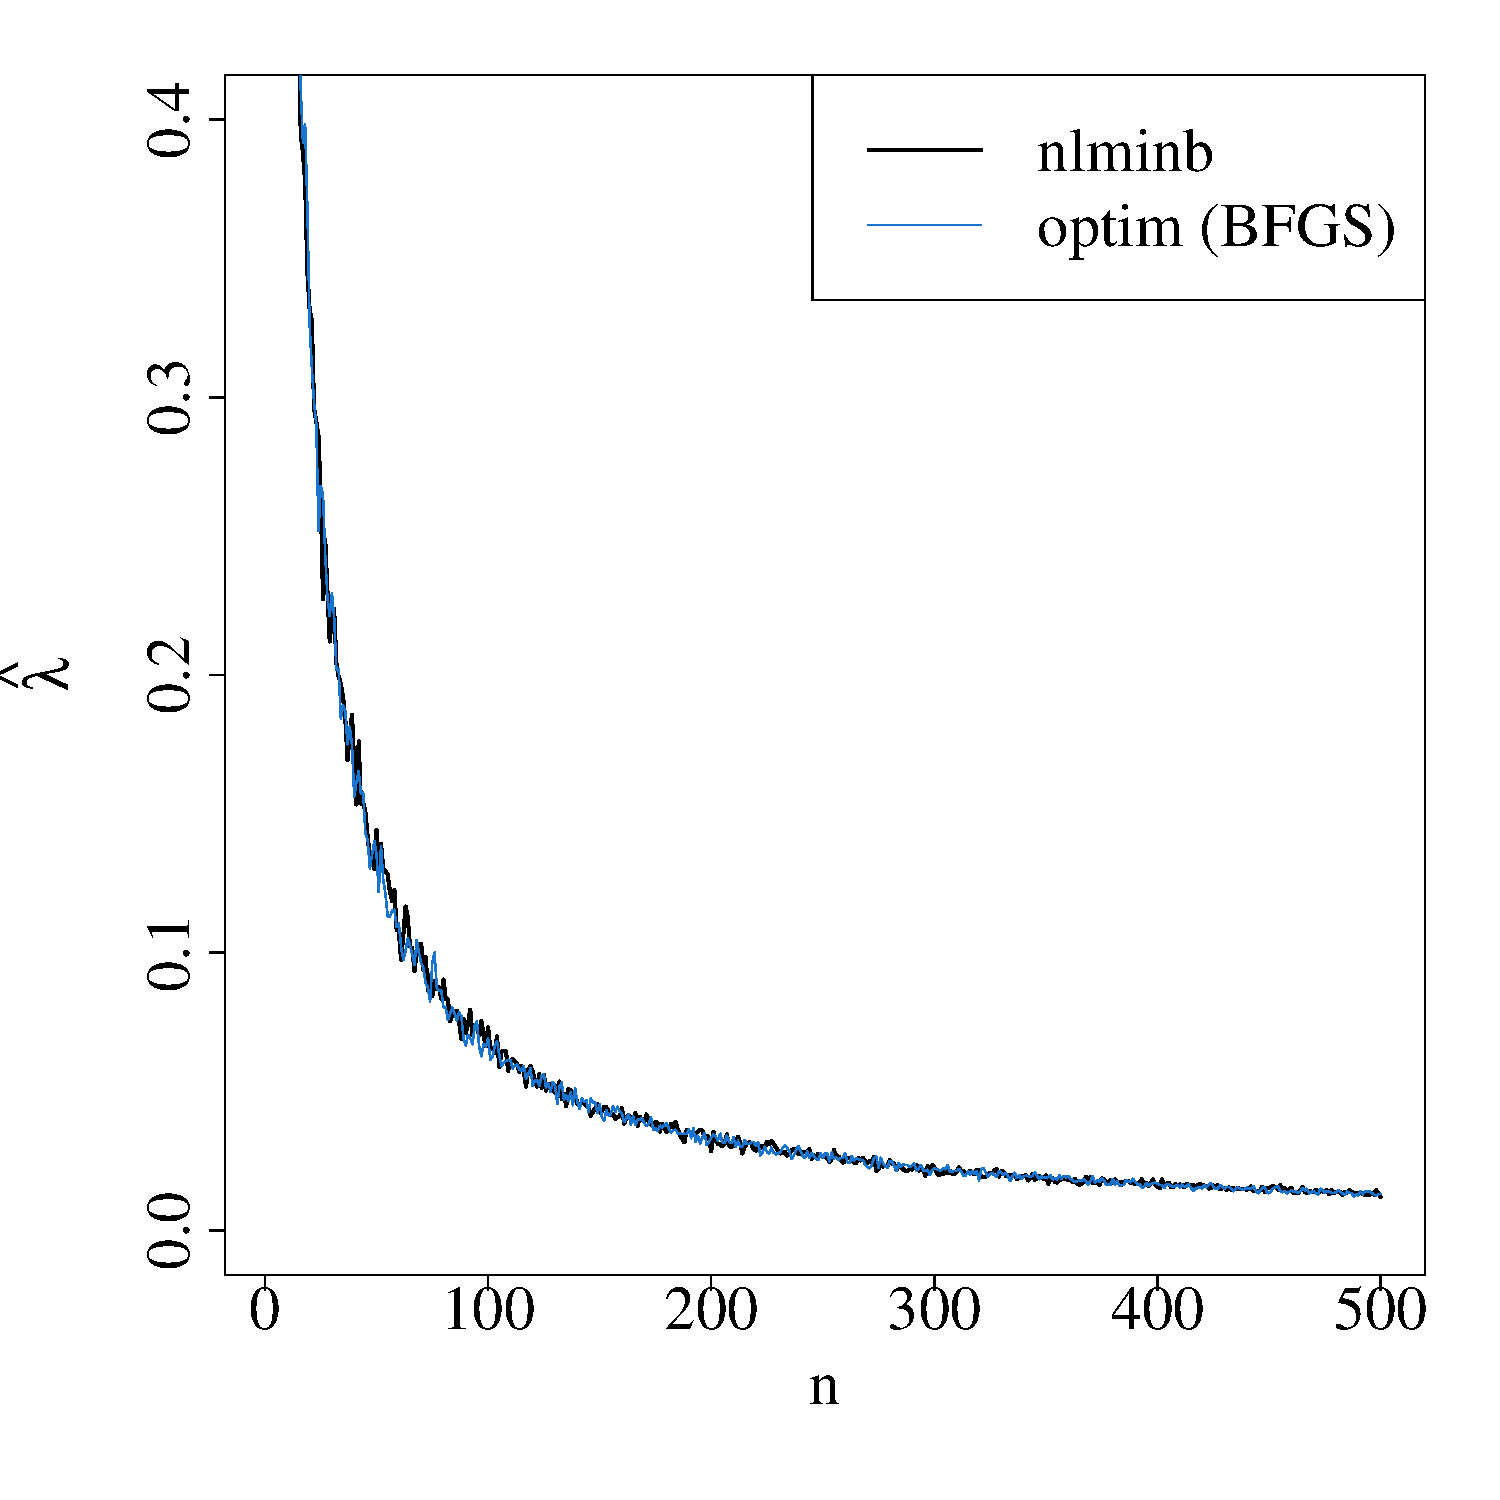
\includegraphics[width=\textwidth]{article-varZIPa}
        \caption{\label{fig:varZIPa}}
    \end{subfigure}
    \begin{subfigure}[h]{0.49\textwidth}
        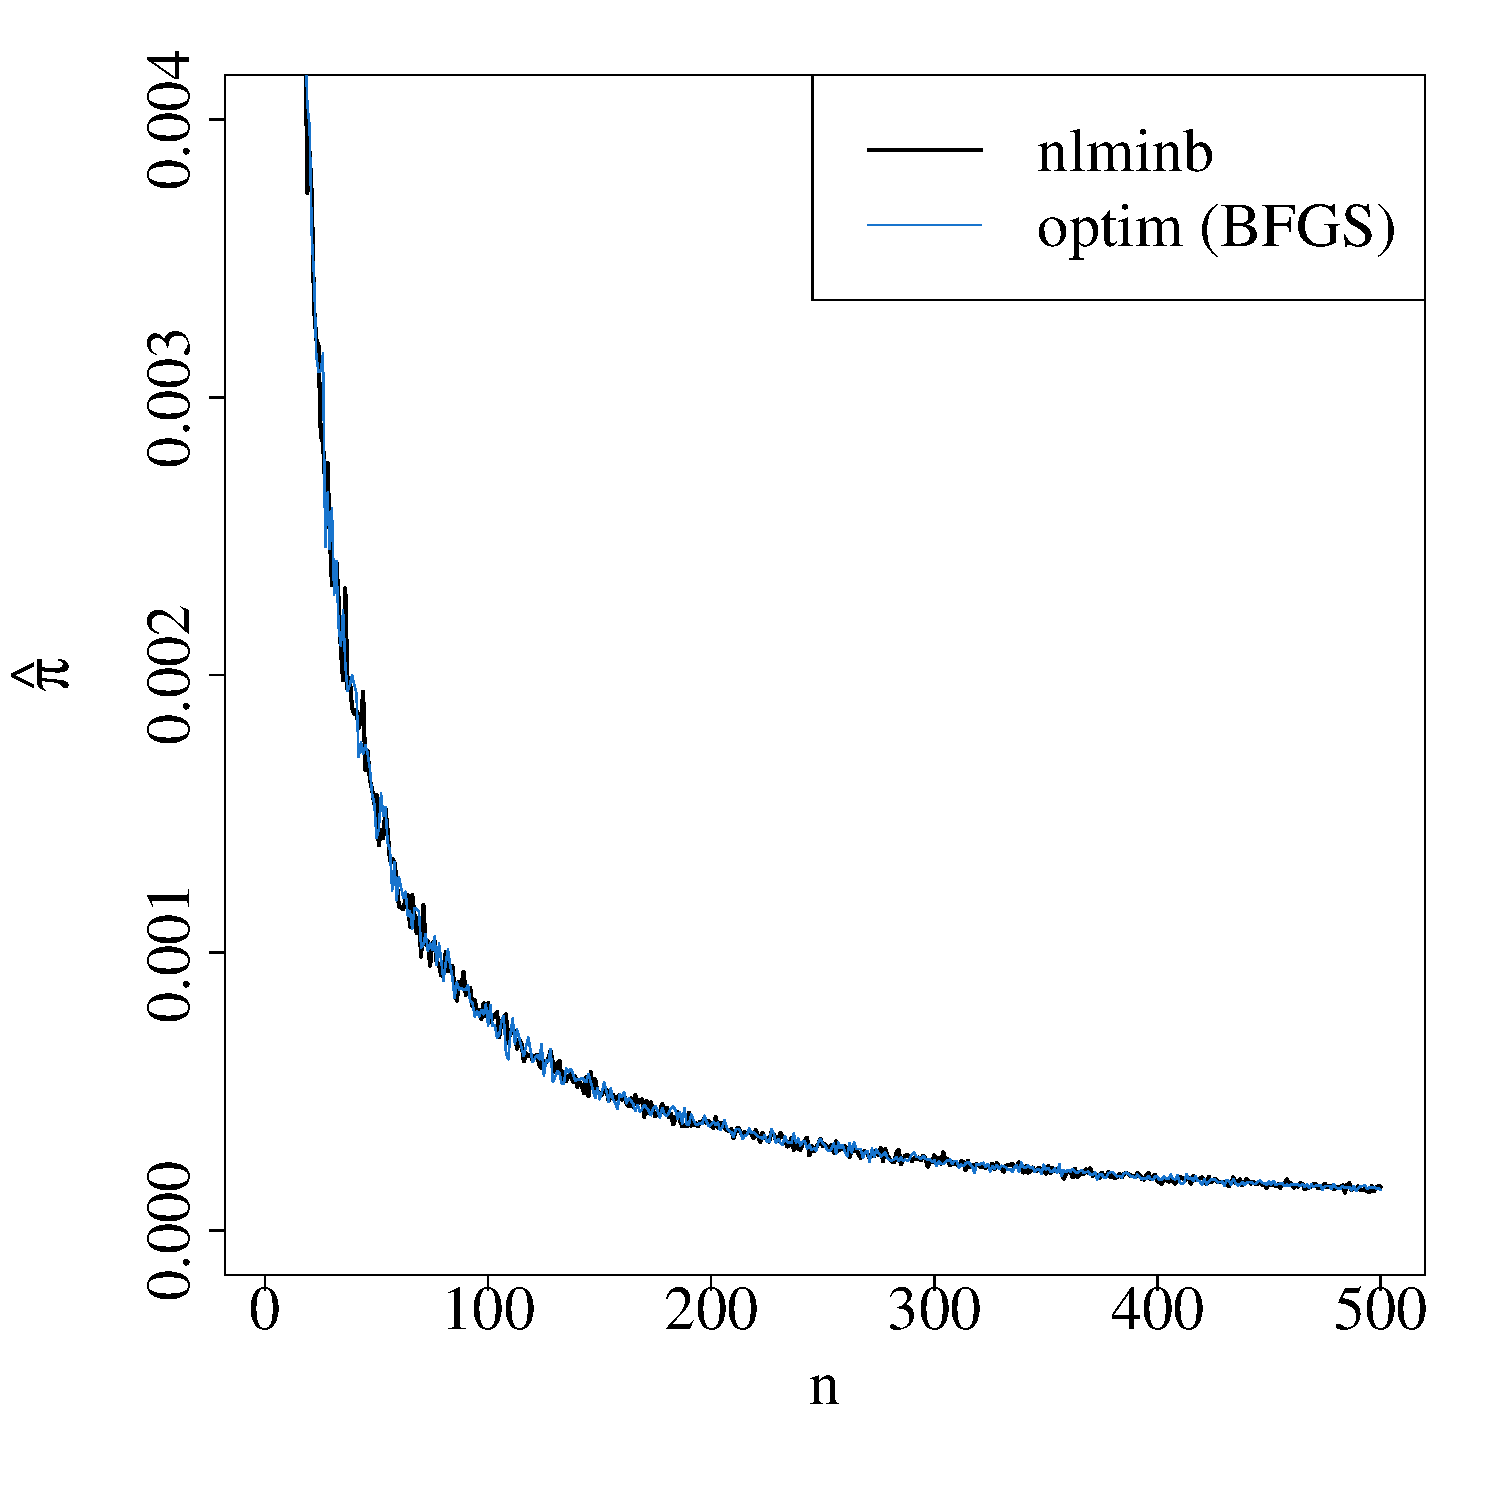
\includegraphics[width=\textwidth]{article-varZIPb}
        \caption{\label{fig:varZIPb}}
    \end{subfigure}
\caption{\label{fig:varZIP} Variance for (a) rate parameter $\hat{\lambda}$ and (b) extra zeros proportion $\hat{\pi}$ versus sample size $n$ in ZIP distribution based on 1000 replications.}
\vspace{-20pt}
\end{figure}

\subsection{EEB distribution}




\begin{figure}[H]
  \vspace{-60pt}
  \centering
    \begin{subfigure}[h]{0.49\textwidth}
        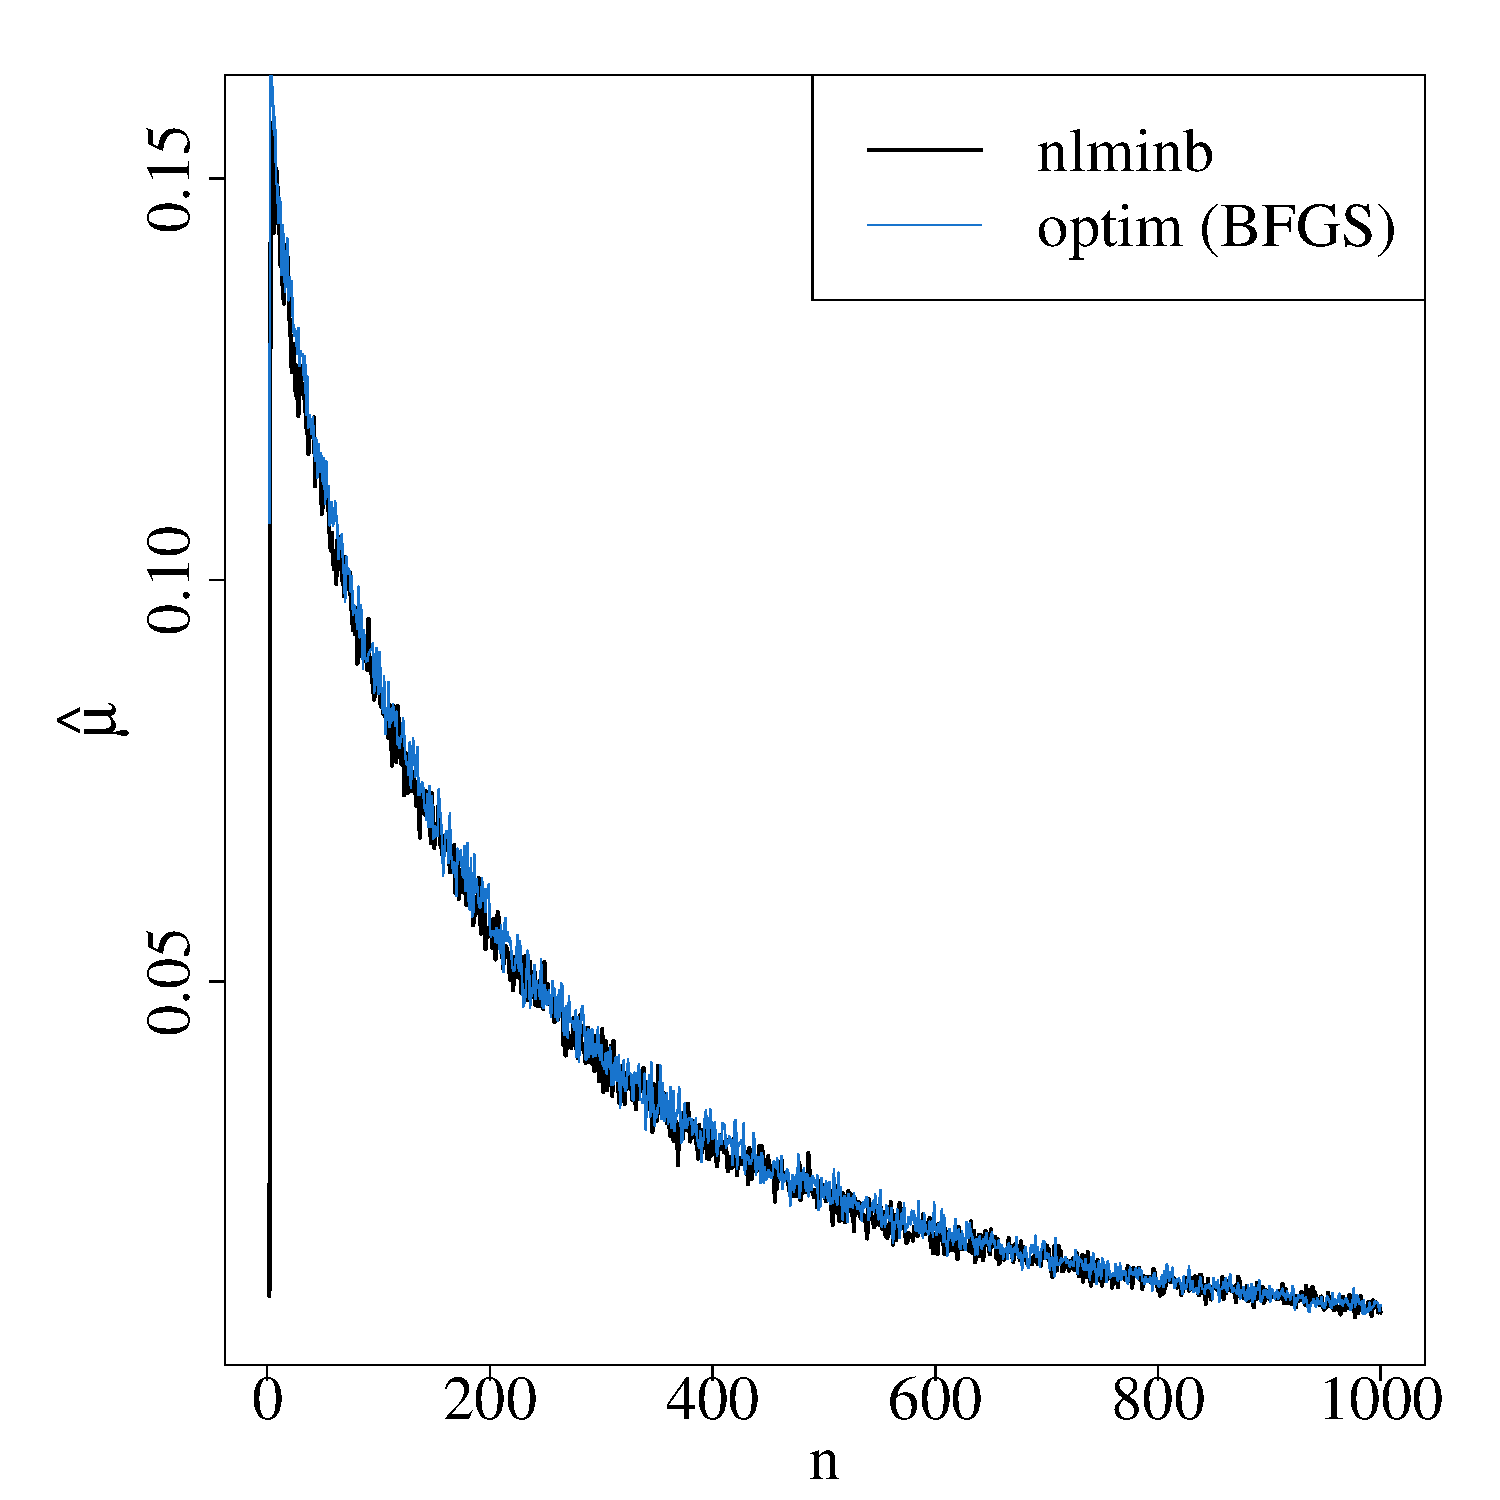
\includegraphics[width=\textwidth]{article-varEEBa}
        \caption{\label{fig:varEEBa}}
    \end{subfigure}
    \begin{subfigure}[h]{0.49\textwidth}
        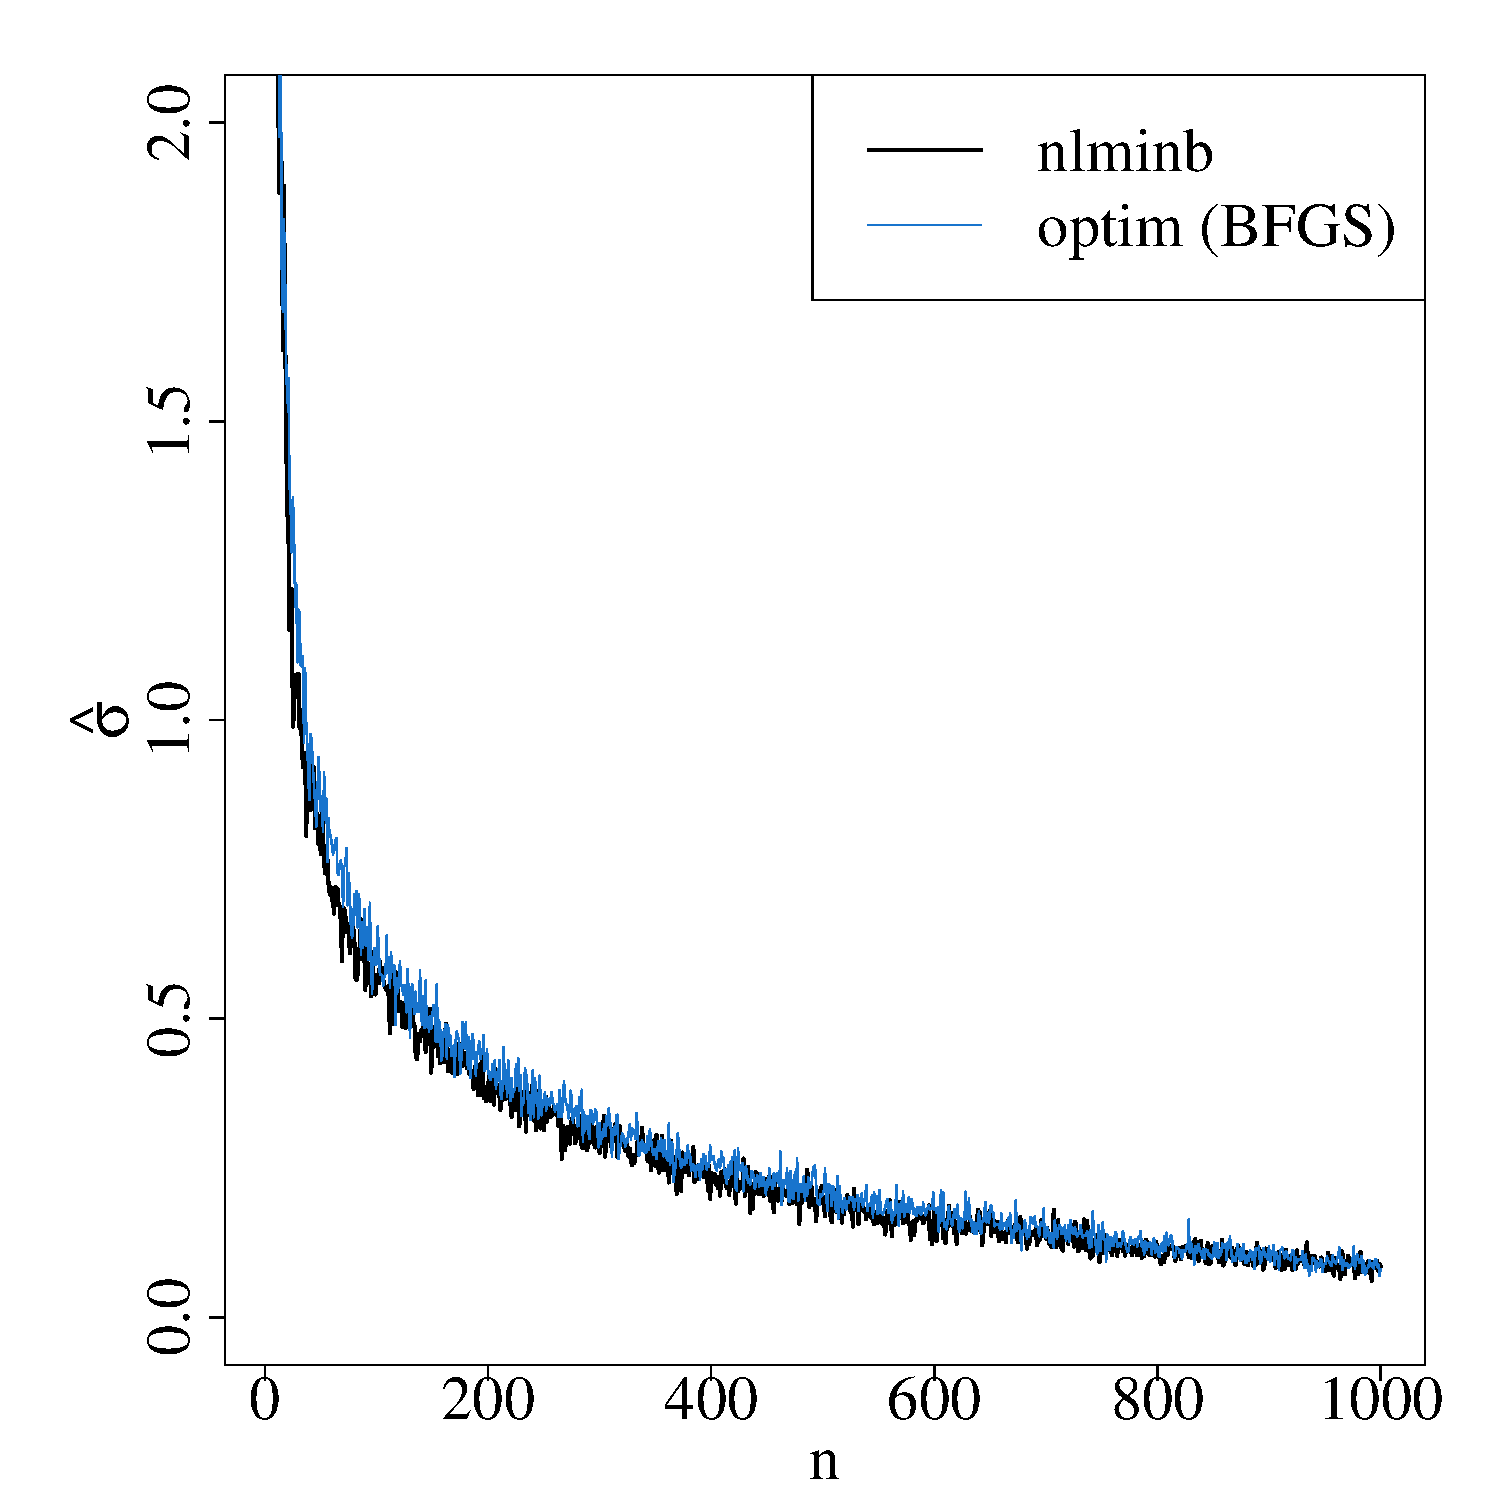
\includegraphics[width=\textwidth]{article-varEEBb}
        \caption{\label{fig:varEEBb}}
    \end{subfigure}
    ~
    \begin{subfigure}[h]{0.49\textwidth}
        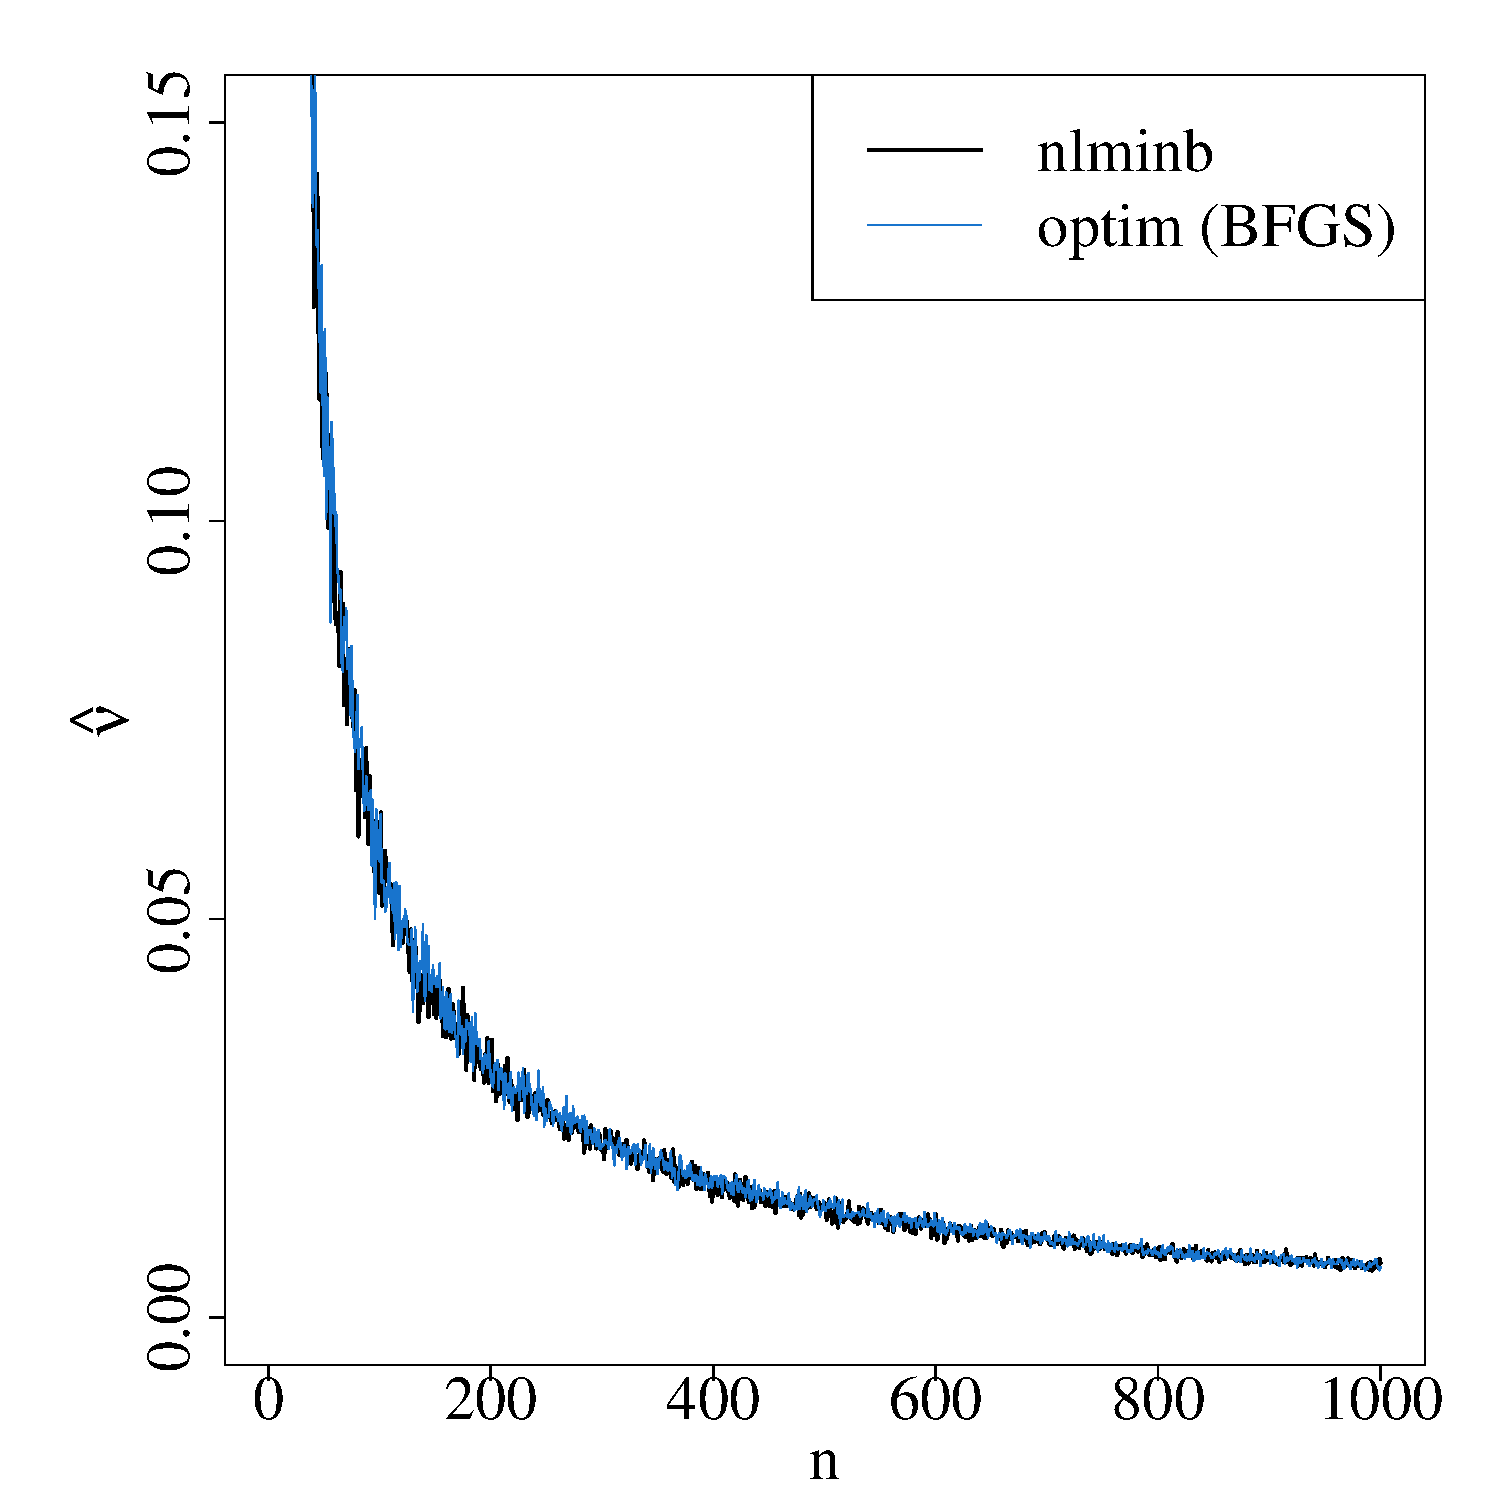
\includegraphics[width=\textwidth]{article-varEEBc}
        \caption{\label{fig:varEEBc}}
    \end{subfigure}
\caption{\label{fig:varEEB} Variance for (a) proportion of successes $\hat{\mu}$, (b) scale parameter $\hat{\sigma}$ and (c) shape parameter $\hat{\tau}$ versus sample size $n$ in EEB distribution based on 1000 replications.}
\vspace{90pt}
\end{figure}

\end{appendix}

%% -----------------------------------------------------------------------------


\end{document}
